%\documentclass[handout]{beamer}
\documentclass{beamer}
\usepackage[utf8]{inputenc}
\usepackage[francais]{babel}
\usepackage[T1]{fontenc}
%\usepackage{multimedia}
\usepackage{graphicx}
\usepackage{hyperref}
\usepackage{algorithm}
\usepackage{algpseudocode}
\floatname{algorithm}{Algorithme} 
\usepackage{listings}
\usepackage[display]{texpower}

%\usetheme[width=100pt]{PaloAlto}
\usetheme[compress]{Ilmenau}
%\usecolortheme{fly}
\setbeamertemplate{frametitle}[default][center]

%\setbeamercovered{transparent}

\title{Proactive : Un middleware open source pour le calcul parallèle}

\author{Veyssier Julien}
\institute{CBGP - INRA}
\date{25 Octobre 2011}
\setbeamertemplate{navigation symbols}{}
%\logo{}
\begin{document}

\begin{frame}
\titlepage
\end{frame}

\begin{frame}
\tableofcontents
\end{frame}

\section[Introduction]{Introduction}
\begin{frame}
	\tableofcontents[currentsection]
\end{frame}

\begin{frame}{Contexte}
\pageTransitionDissolve
	\begin{columns}
	\begin{column}[l]{0.5\linewidth}
        \begin{columns}
        \begin{column}[l]{0.5\linewidth}
        \begin{figure}
            %[!bh]
            \centering
            
\includegraphics[scale=0.32]{cbgp.png}
            %\caption{Architecture autour d'un CDN}
        \end{figure}
        \end{column}
        \begin{column}[r]{0.5\linewidth}
        \begin{figure}
            %[!bh]
            \centering
            
\includegraphics[scale=0.32]{cocci.png}
            %\caption{Architecture autour d'un CDN}
        \end{figure}
        \end{column}
        \end{columns}
        \vspace{1cm}
	\begin{block}{Objectifs}<2->
			\begin{itemize}
                    %decouplage .. .
                \item Refonte de DIYABC
				\item Implémentation de l'interface graphique
                \item Interfaçage avec des outils de calcul parallèle
			\end{itemize}
					
		\end{block}

	\end{column}
	\begin{column}[r]{0.5\linewidth}
	\begin{exampleblock}{Activités du laboratoire}<1->
			\begin{itemize}
				\item Génétique des population
                \item Systématique
                \item Écologie
			\end{itemize}
					
		\end{exampleblock}
	\begin{block}{Moyens matériels}<3->
			\begin{itemize}
                \item Cluster local (SGE)
				\item Machines personnelles des chercheurs
                \item Postes de travail de l'administration
			\end{itemize}
					
		\end{block}
	\end{column}
	\end{columns}
\end{frame}

\begin{frame}{Exploration des outils plus polyvalents que SGE}
    Constat : architectures trop rigides % cluster only
	\begin{columns}
	\begin{column}[l]{0.3\linewidth}
    \begin{block}{Projets}
        \begin{itemize}
                % alex a utilisé diane, bien mais manque d'outils qui facilitent la vie
            \item<2-> Diane
                % orienté grilles
            \item<3-> Wisdom
                % example de projet qui ne fourni pas son programme
            \item<4-> OurGrid
            \item<5-> Proactive
        \end{itemize}
    \end{block}
	\end{column}
	\begin{column}[r]{0.6\linewidth}
    \begin{exampleblock}{Particularité}
        \begin{itemize}
            \item<2-> Peu d'outils annexe
            \item<3-> Orienté vers les grilles de calcul
            \item<4-> Programmes non fournis
            \item<5-> Découplé et polyvalent
        \end{itemize}
    \end{exampleblock}
	\end{column}
	\end{columns}
\end{frame}

%\begin{frame}{Proactive}
%    Exploration des possibilités pour une éventuelle intégration au CBGP
%\end{frame}

\section[Fonctionnement]{Fonctionnement de Proactive}
\begin{frame}
	\tableofcontents[currentsection]
\end{frame}
\begin{frame}{Vue d'ensemble}
    \begin{itemize}
        \item Langage de programmation $\Longrightarrow$ Java + Bash/Batch
        \item Portable
        \item Supporte un environnement hétérogène (Unix*, Windows)% scripts de selection
        \item Différents niveaux d'utilisation (de débutant à expert) % simple, avancé
        \item Différentes interfaces : GUI, CLI, API (intégration dans votre propre application)
        \item Extensible et découplé
            % decouplé : chaque executable est indépendant et ne nécessite pas forcément l'exécution des autres
            %    => choix des composants en fction des besoins
            % extensible : logiciel libre sous affero GPL que l'on peut améliorer grace aux libs fournies
    \end{itemize}

\end{frame}
\subsection{Architecture}
\begin{frame}
	\tableofcontents[currentsubsection]
\end{frame}
\begin{frame}{Architecture}
	\begin{columns}
	\begin{column}[l]{0.5\linewidth}
        \begin{figure}
            %[!bh]
            \centering
            %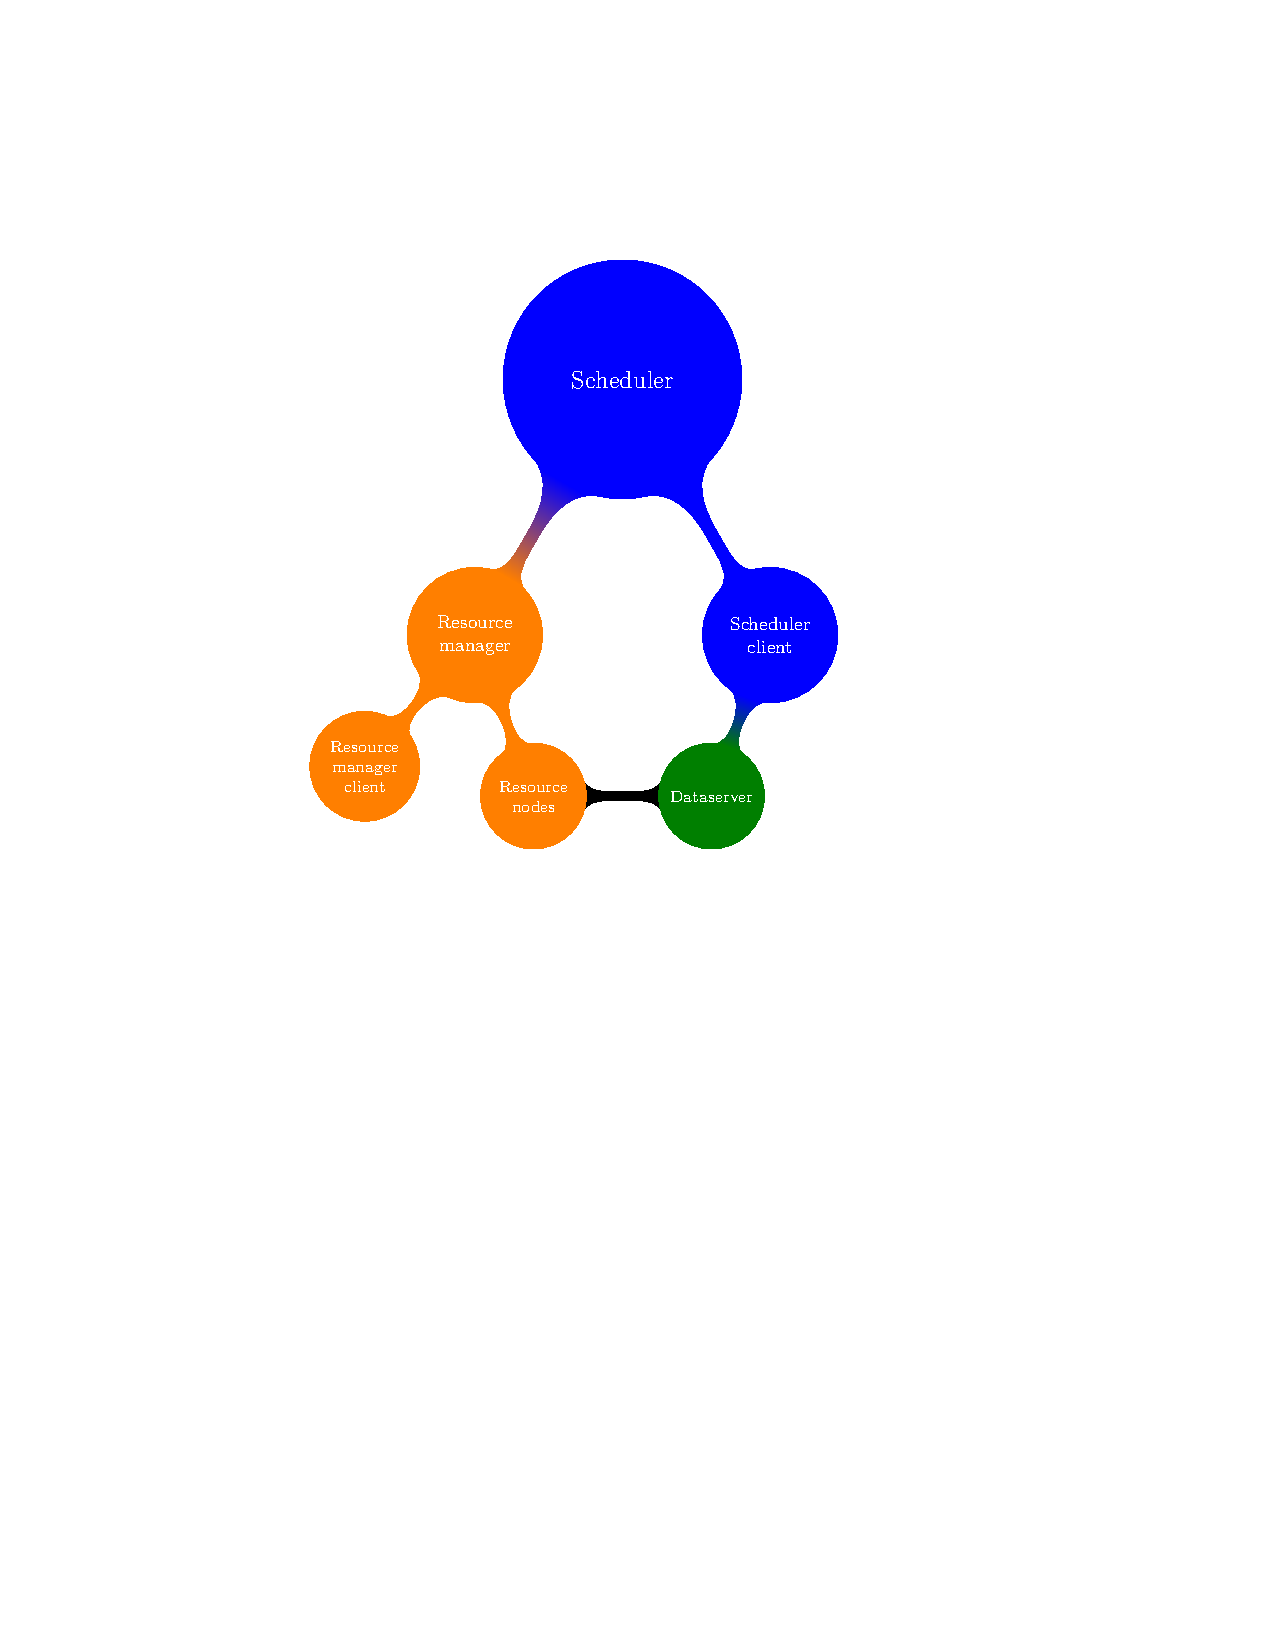
\includegraphics[trim=4cm 13cm 2cm 5cm,scale=0.48]{netmap_abs.pdf}
            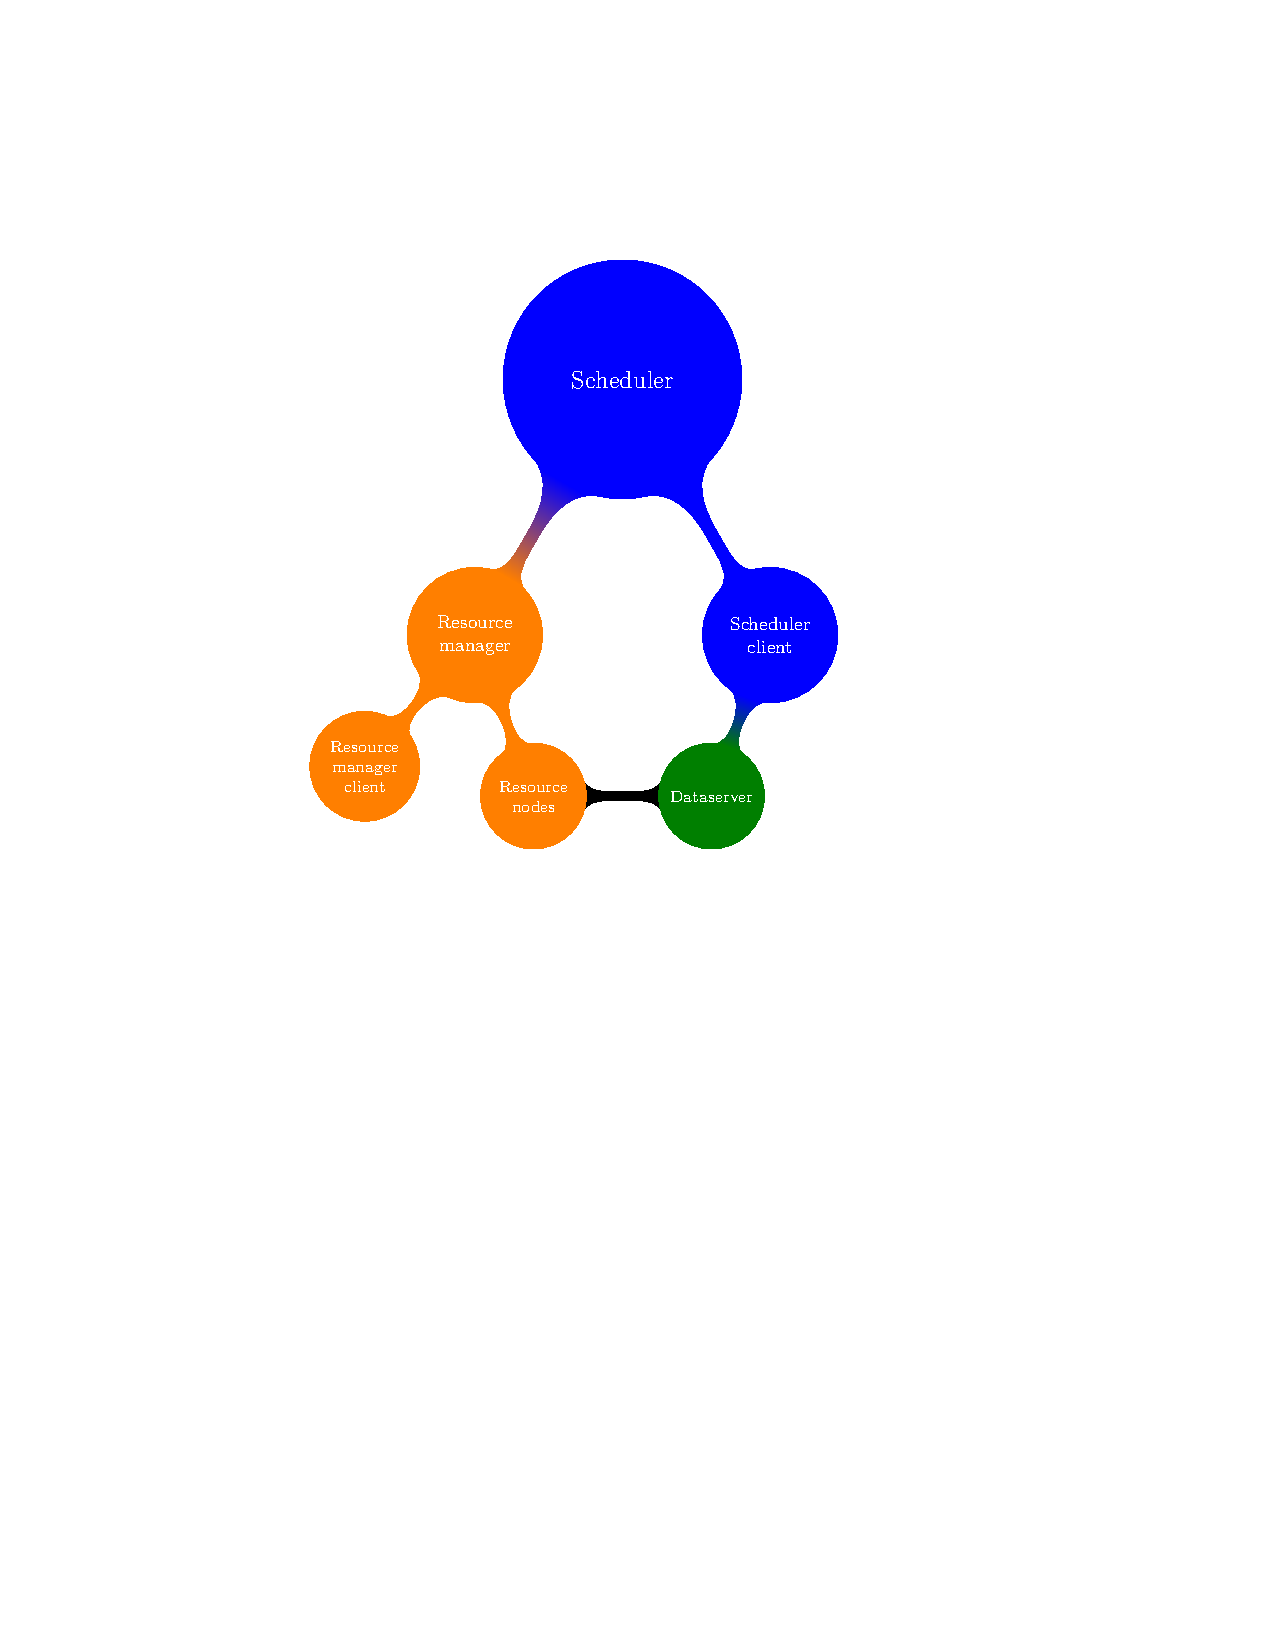
\includegraphics[trim=5.5cm 14.3cm 2cm 6.3cm,scale=0.69]{netmap_abs.pdf}
            %\caption{Communication dans Proactive}
        \end{figure}
	\end{column}
    \setbeamercolor{block title}{fg=white,bg=orange}   
    \setbeamercolor{block body}{fg=black,bg=orange!30}
    \setbeamercolor{block title alerted}{fg=white,bg=blue}   
    \setbeamercolor{block body alerted}{fg=black,bg=blue!30}
    \setbeamercolor{block title example}{fg=white,bg=green!50!black}   
    \setbeamercolor{block body example}{fg=black,bg=green!15}
	\begin{column}[r]{0.5\linewidth}
        \begin{block}{Resource management}
            Gestion des noeuds de calcul
        \end{block}
        \begin{alertblock}{Scheduling}
             Gestion de la politique d'ordonnancement et de la soumission des calculs
        \end{alertblock}
        \begin{exampleblock}{Data management}
            Transmission des données
        \end{exampleblock}
        
	\end{column}
	\end{columns}
\end{frame}

\subsection{Composants}
\begin{frame}
	\tableofcontents[currentsubsection]
\end{frame}
\begin{frame}{Composants}
	\begin{columns}
	\begin{column}[l]{0.5\linewidth}
        \begin{figure}
            %[!bh]
            \centering
            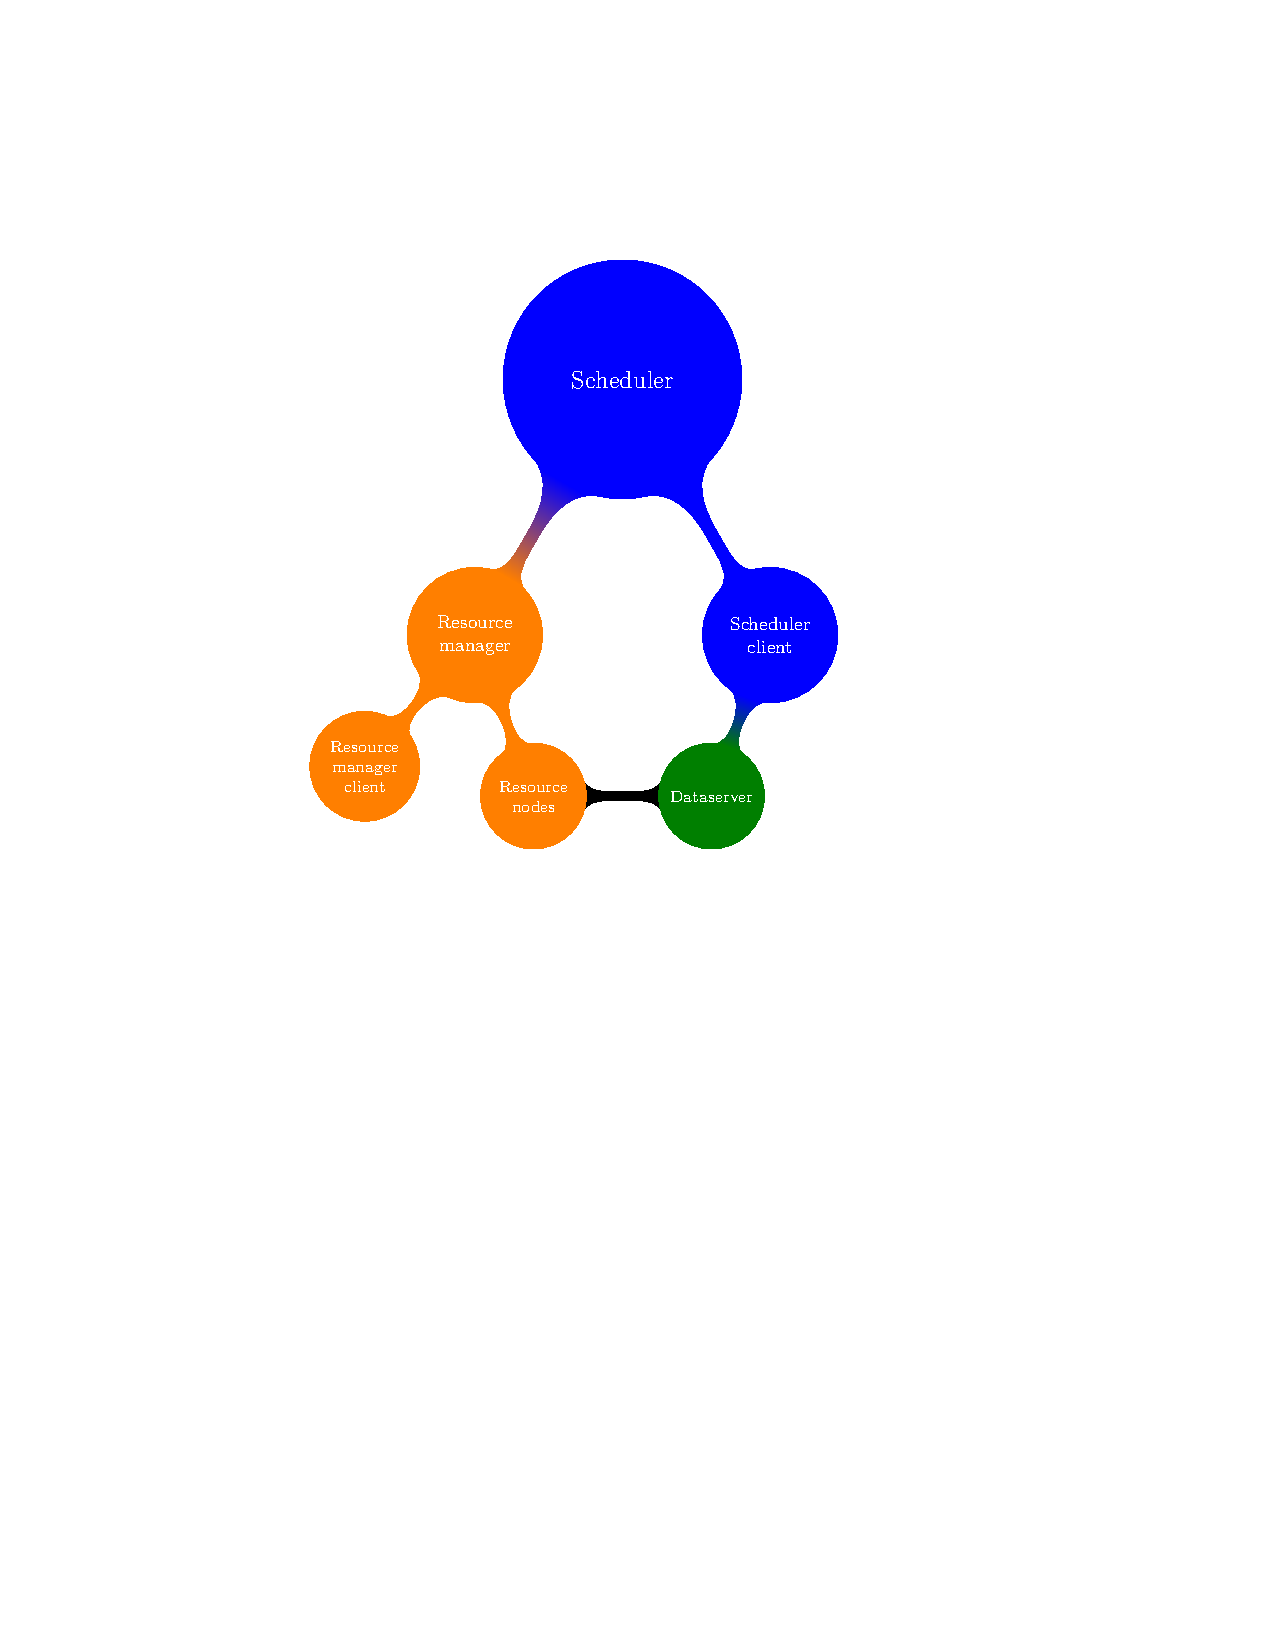
\includegraphics[trim=5.5cm 14.3cm 2cm 6.3cm,scale=0.69]{netmap_abs.pdf}
            %\caption{Communication dans Proactive}
        \end{figure}
	\end{column}
    \setbeamercolor{block title}{fg=white,bg=orange}   
    \setbeamercolor{block body}{fg=black,bg=orange!30}
    \setbeamercolor{block title alerted}{fg=white,bg=blue}   
    \setbeamercolor{block body alerted}{fg=black,bg=blue!30}
    \setbeamercolor{block title example}{fg=white,bg=green!50!black}   
    \setbeamercolor{block body example}{fg=black,bg=green!15}
	\begin{column}[r]{0.5\linewidth}
        
        \begin{block}{Resource management}
            \begin{itemize}
                \item Resource node
                \item Resource manager
                \item Resource manager client
            \end{itemize}
            %Accepte et traite des calculs
        \end{block}
        \begin{alertblock}{Scheduling}
            \begin{itemize}
                \item Scheduler
                \item Scheduler client
            \end{itemize}
            %Attend des calculs et les affecte à des noeuds de calcul
        \end{alertblock}
        \begin{exampleblock}{Data management}
            \begin{itemize}
                \item Dataserver
            \end{itemize}
            %Transmet les données liées aux calculs
        \end{exampleblock}
        
	\end{column}
	\end{columns}
\end{frame}

\begin{frame}{Resource management}
	\begin{columns}
	\begin{column}[l]{0.5\linewidth}
        \only<1>{\begin{figure}
            %[!bh]
            \centering
            %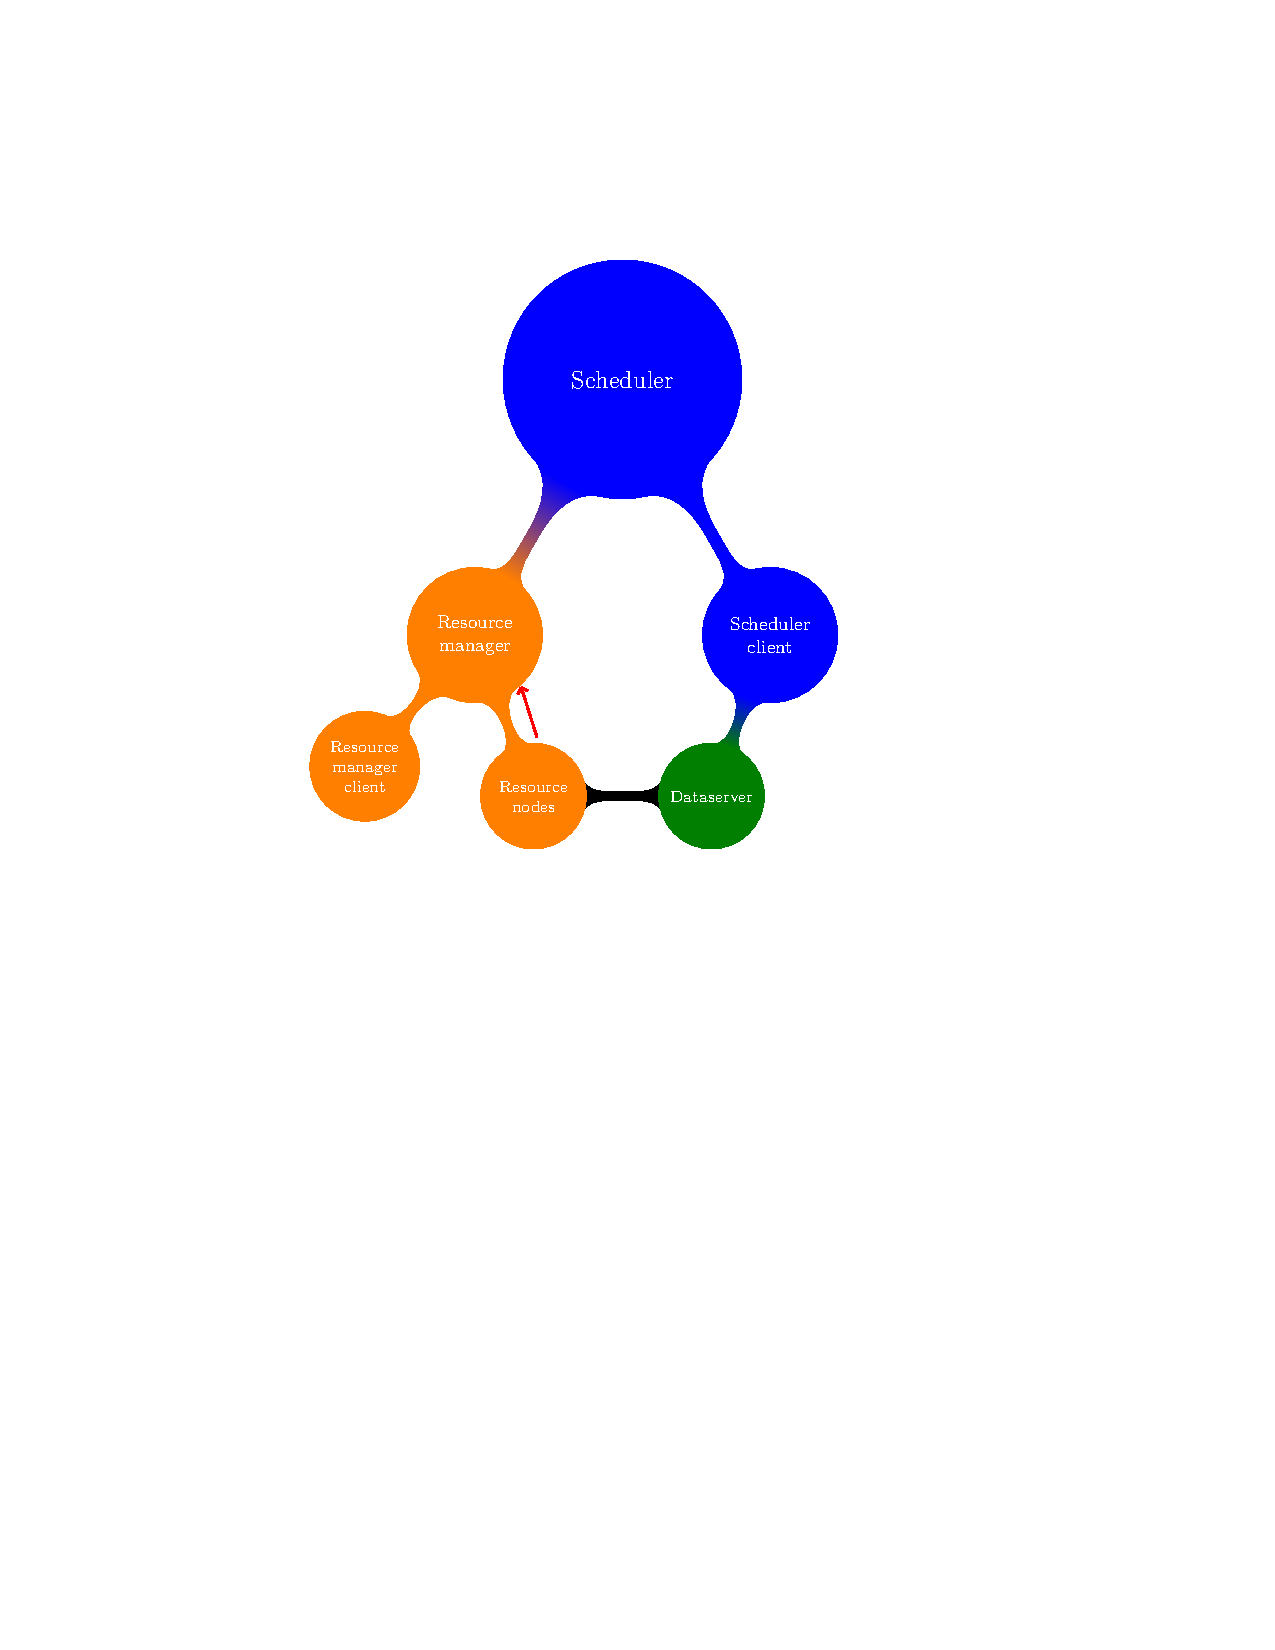
\includegraphics[trim=4cm 13cm 2cm 5cm,scale=0.48]{node_declaration.pdf}
            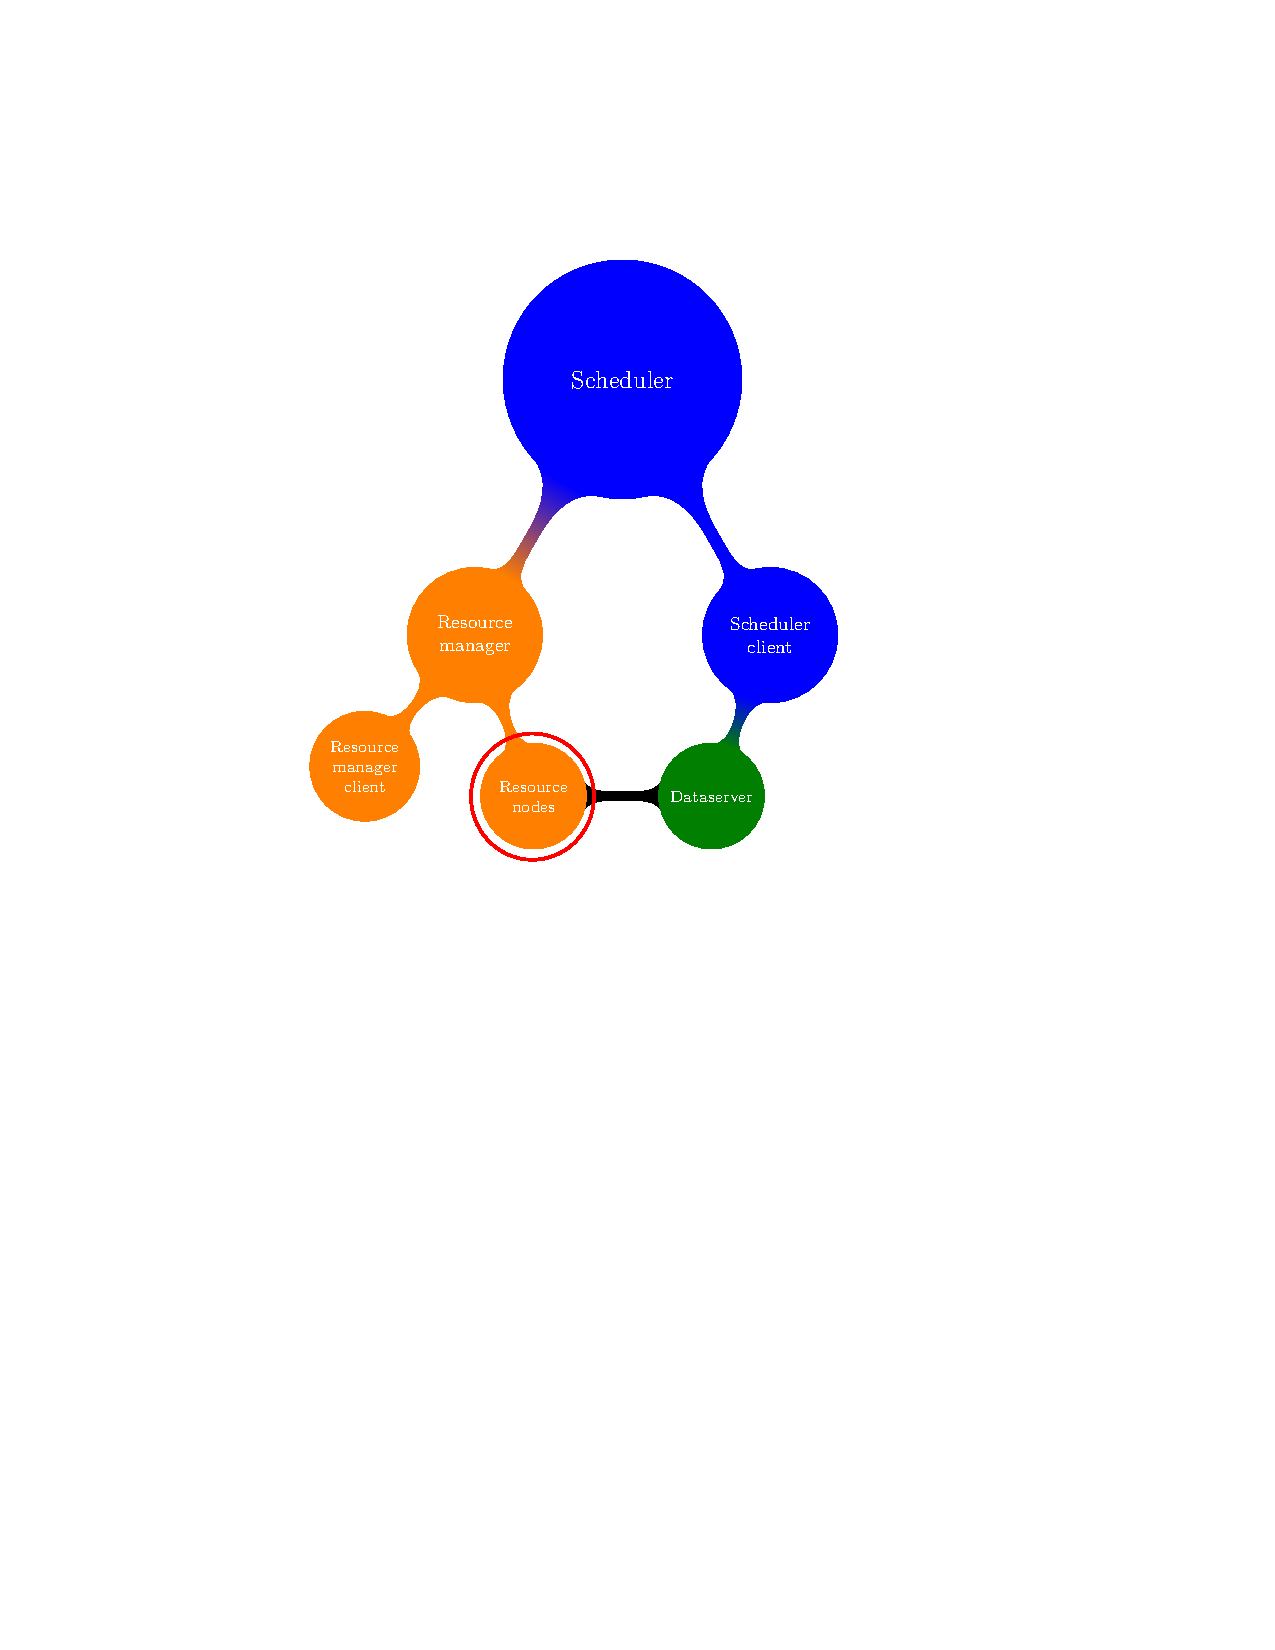
\includegraphics[trim=5.5cm 14.3cm 2cm 6.3cm,scale=0.69]{rn.pdf}
            %\caption{Communication dans Proactive}
        \end{figure}
        }
        \only<2>{\begin{figure}
            %[!bh]
            \centering
            %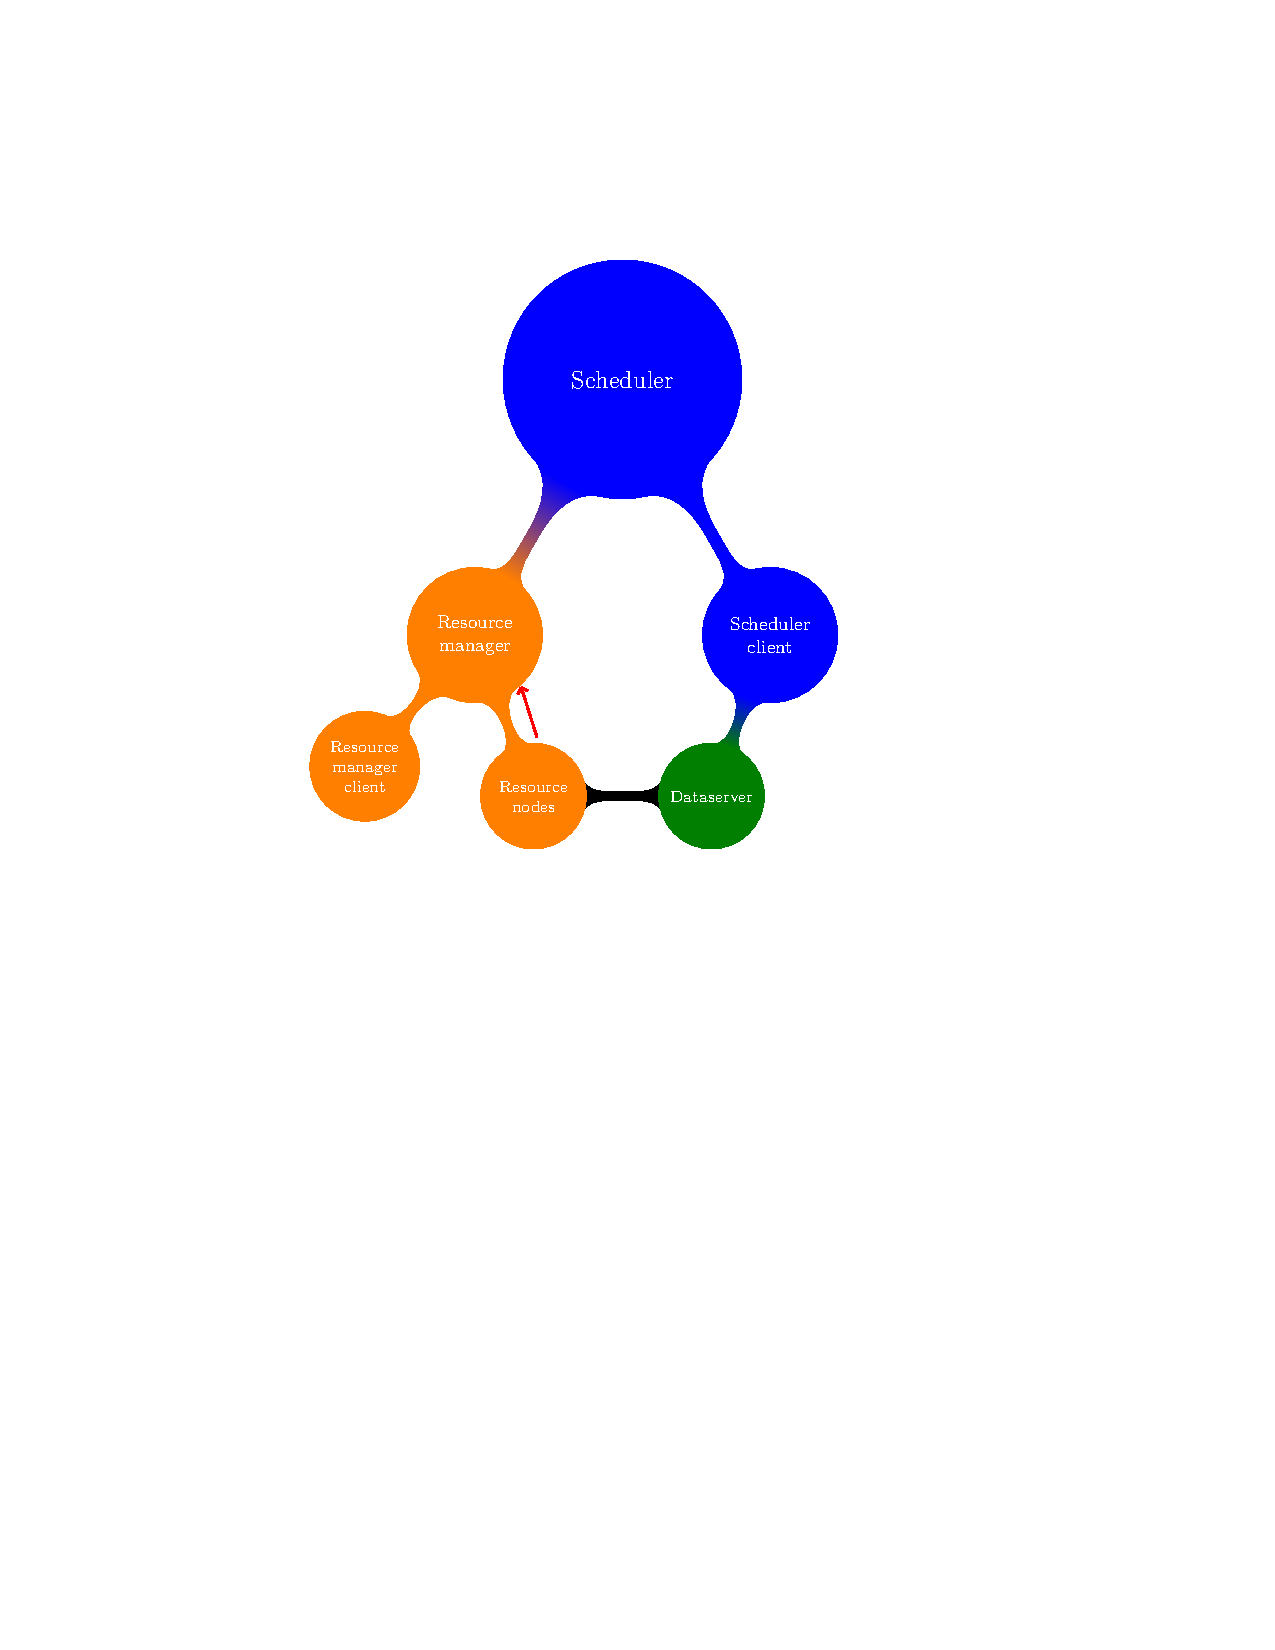
\includegraphics[trim=4cm 13cm 2cm 5cm,scale=0.48]{node_declaration.pdf}
            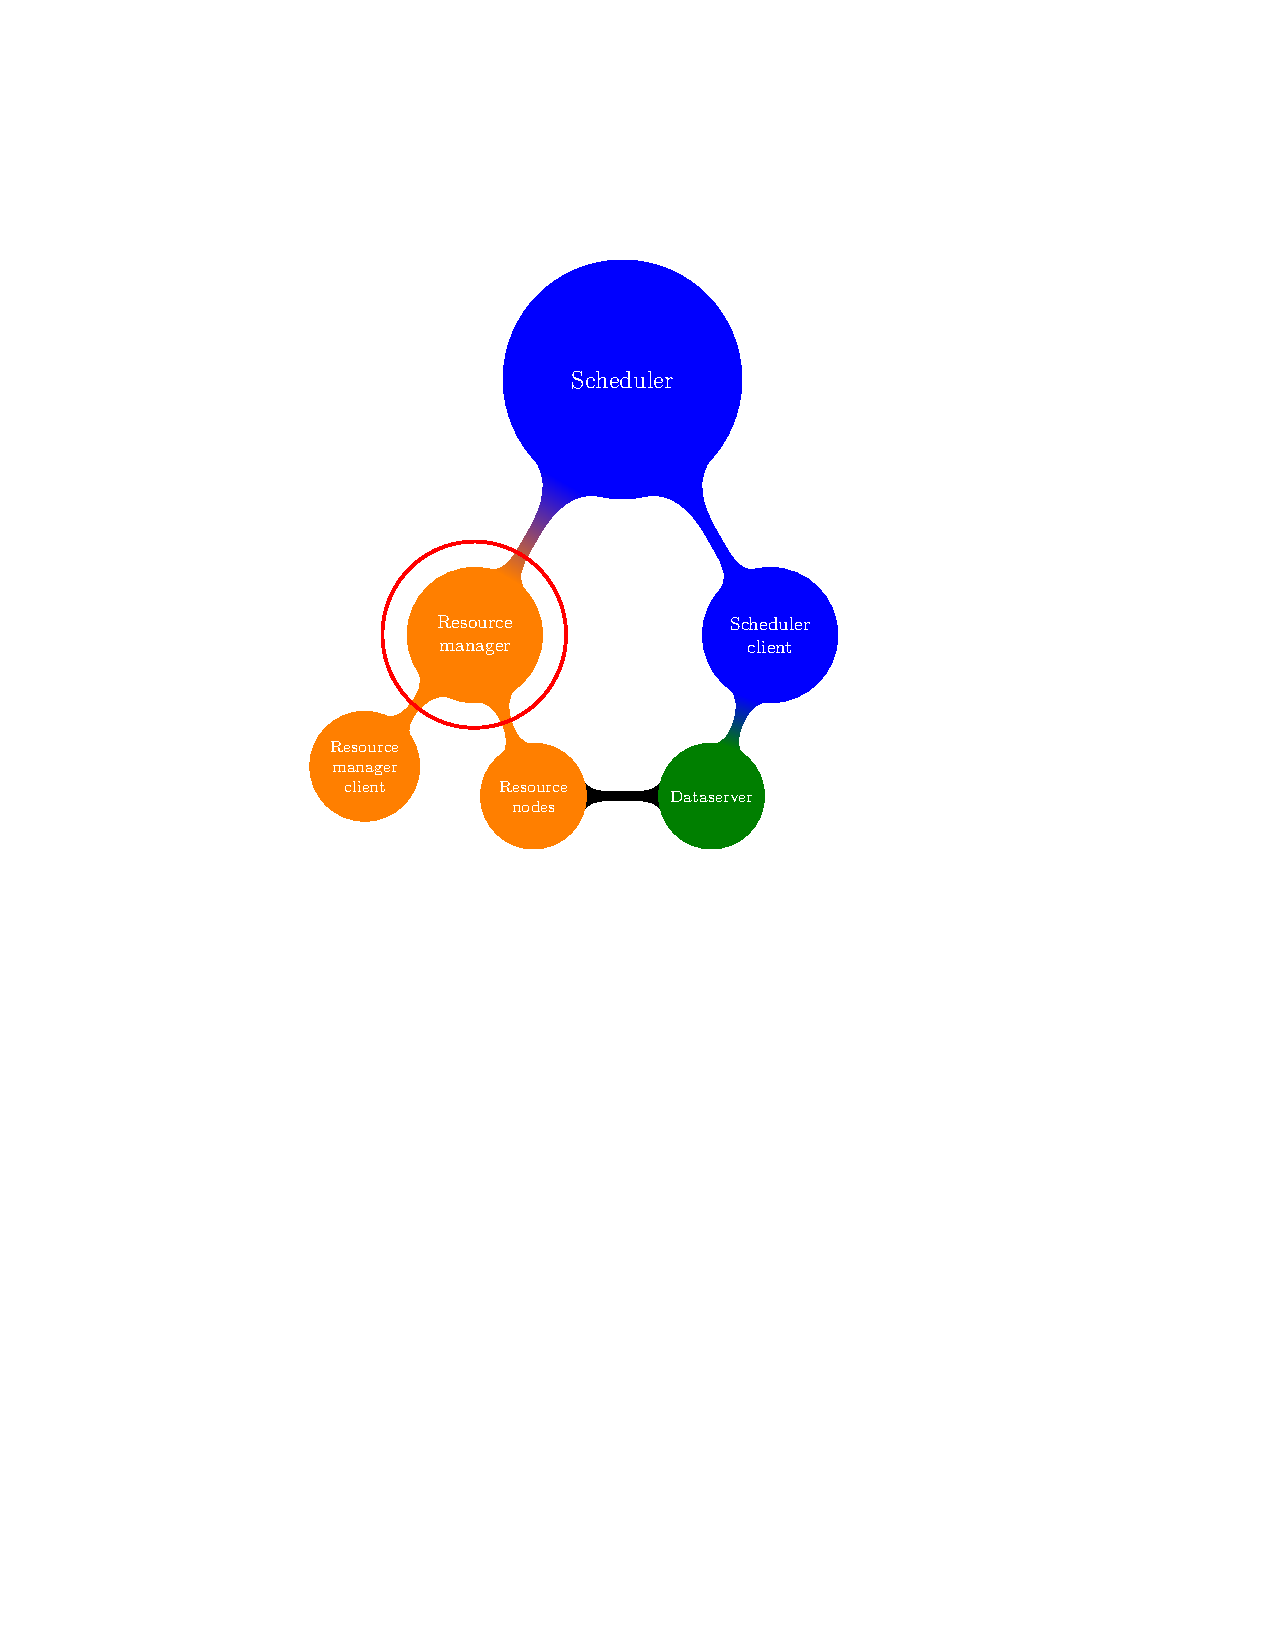
\includegraphics[trim=5.5cm 14.3cm 2cm 6.3cm,scale=0.69]{rm.pdf}
            %\caption{Communication dans Proactive}
        \end{figure}
        }
        \only<3>{\begin{figure}
            %[!bh]
            \centering
            %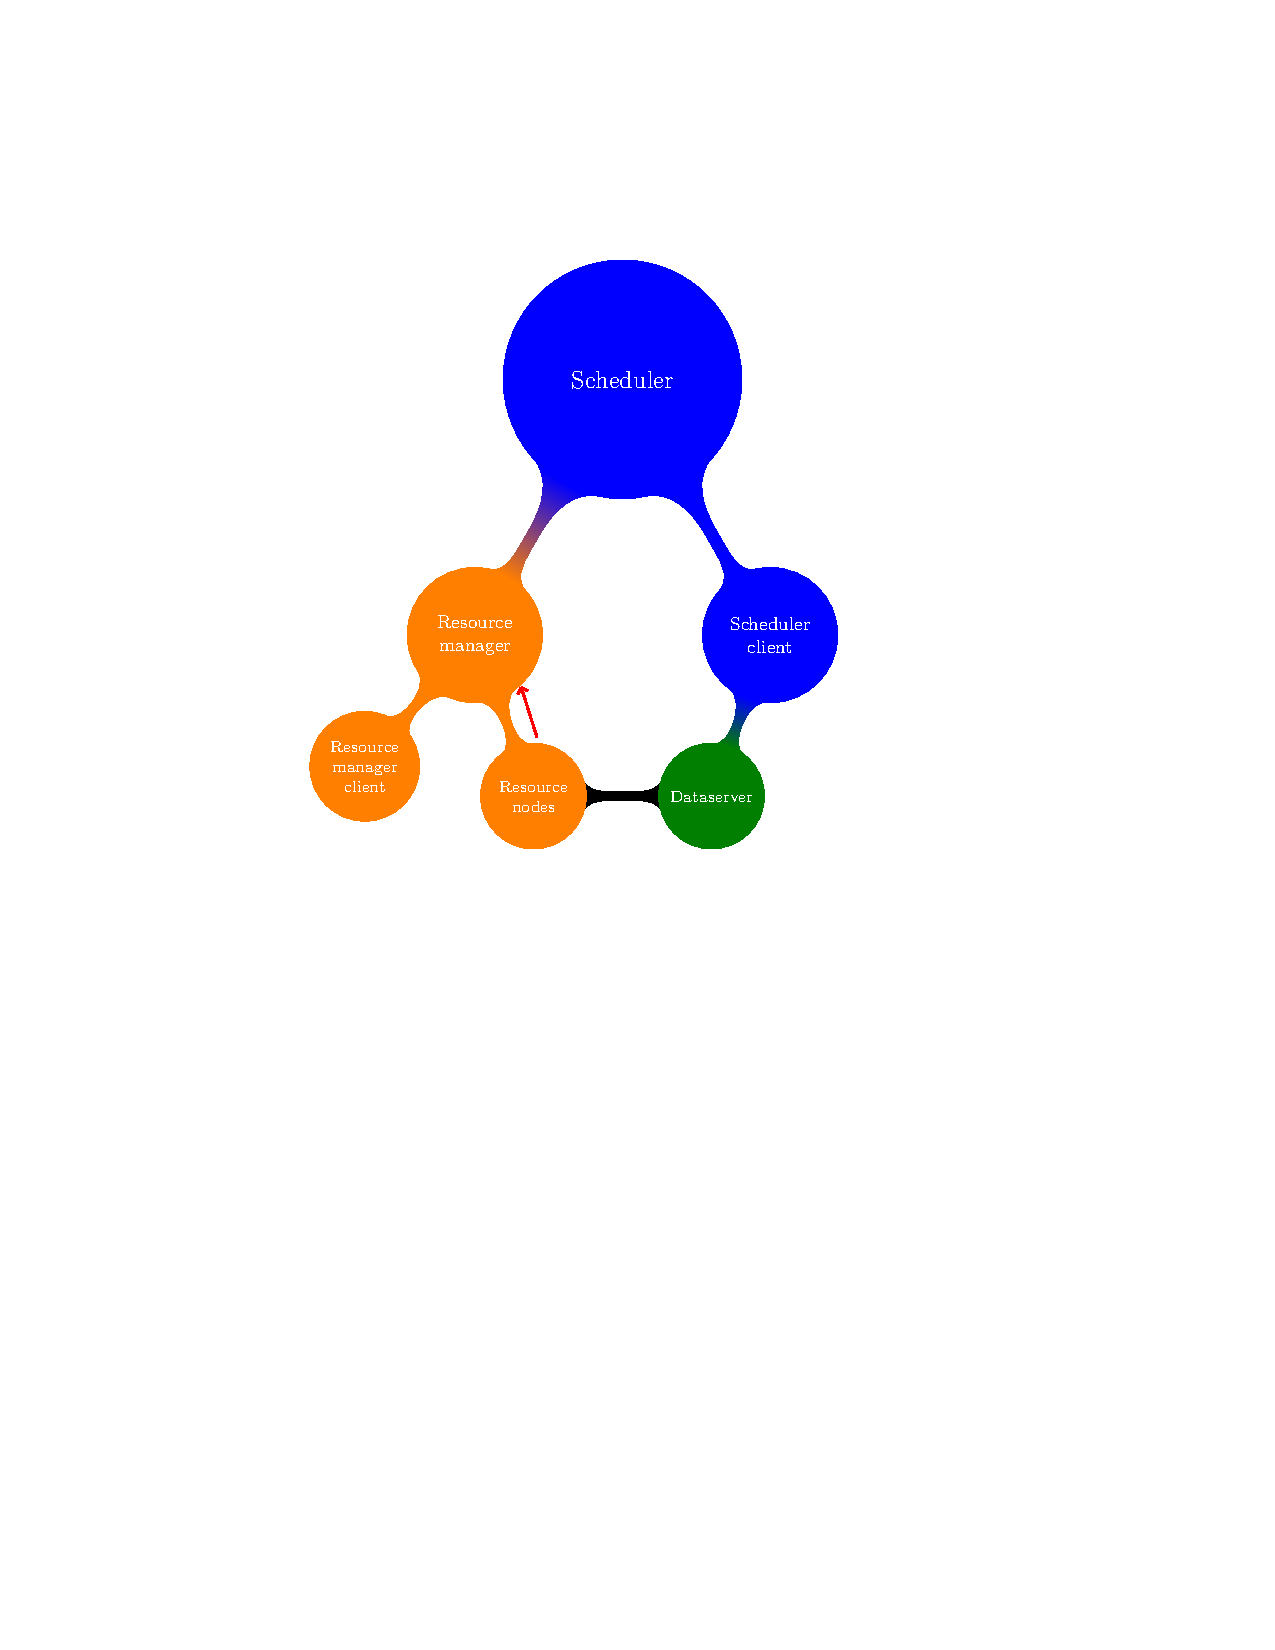
\includegraphics[trim=4cm 13cm 2cm 5cm,scale=0.48]{node_declaration.pdf}
            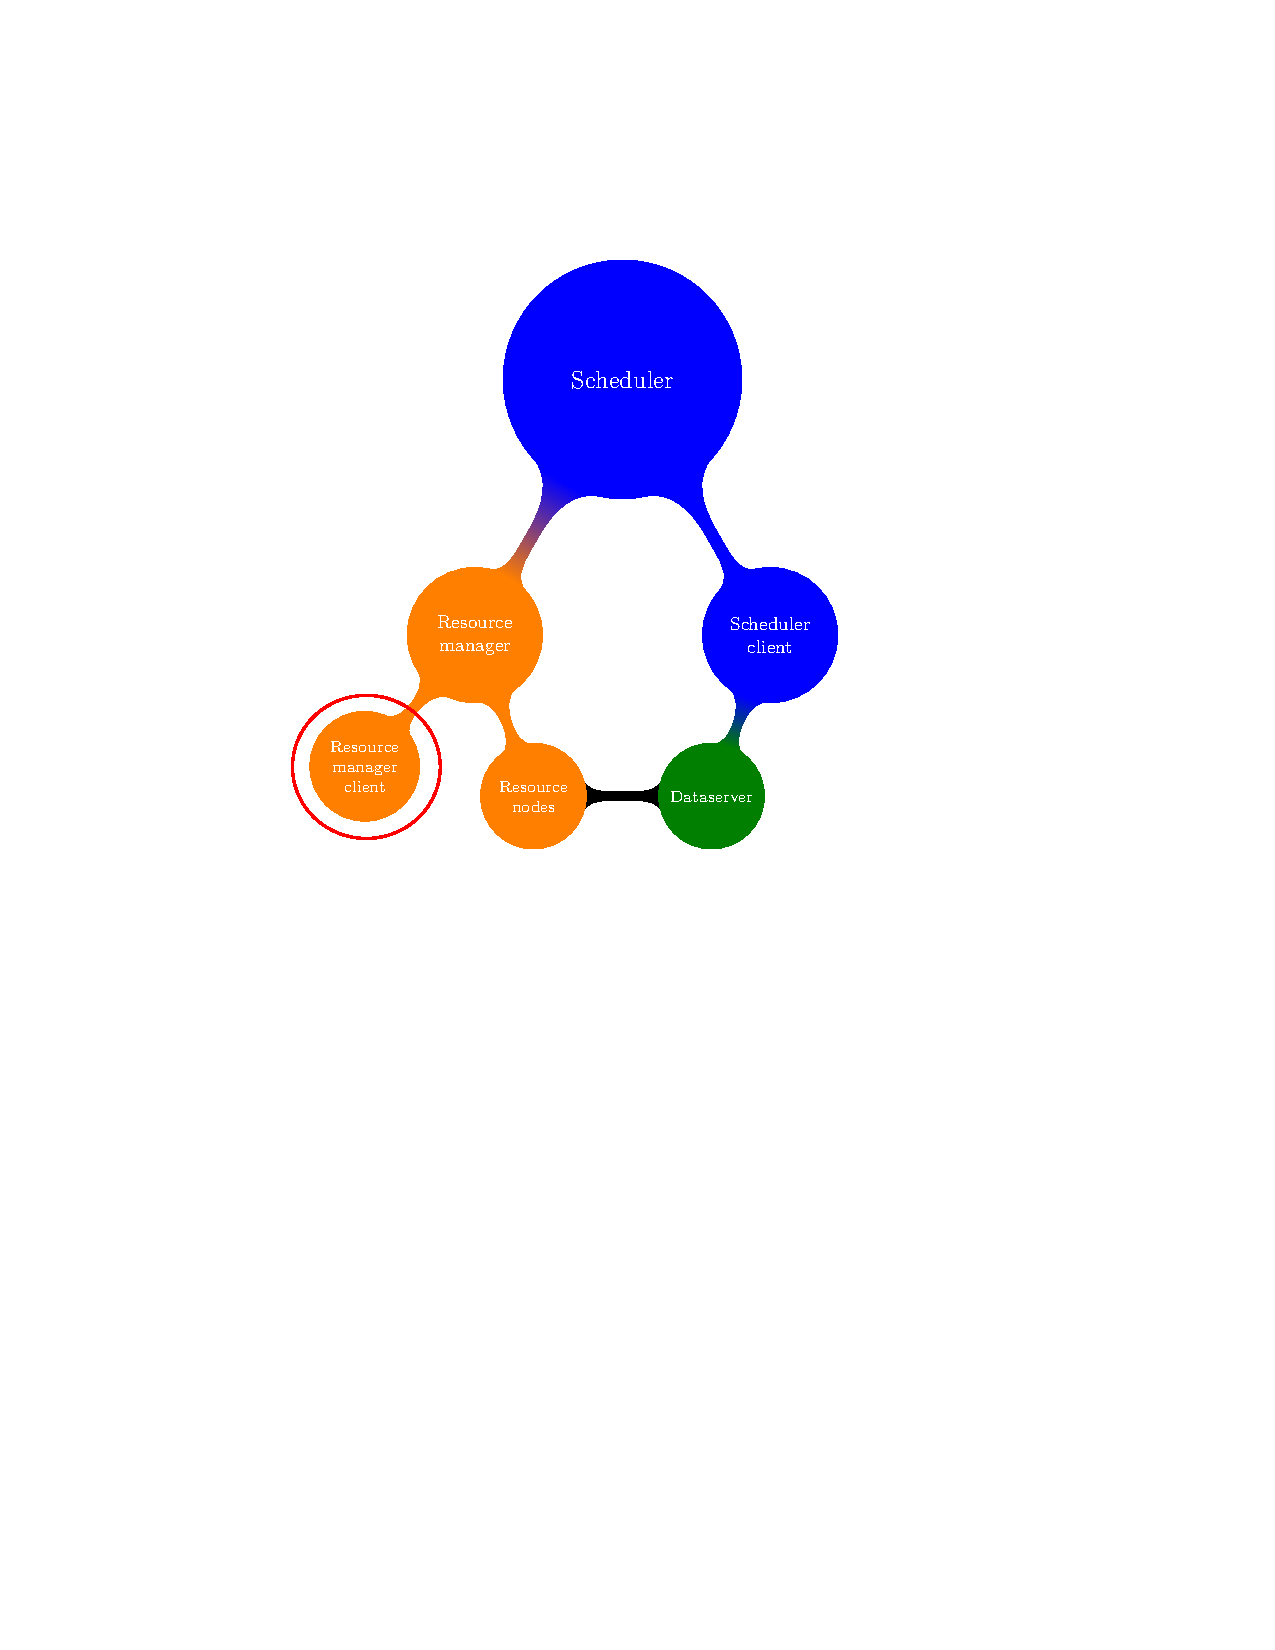
\includegraphics[trim=5.5cm 14.3cm 2cm 6.3cm,scale=0.69]{rmc.pdf}
            %\caption{Communication dans Proactive}
        \end{figure}
        }
	\end{column}
    \setbeamercolor{block title}{fg=white,bg=orange}   
    \setbeamercolor{block body}{fg=black,bg=orange!30}
    \setbeamercolor{block title alerted}{fg=white,bg=blue}   
    \setbeamercolor{block body alerted}{fg=black,bg=blue!30}
	\begin{column}[r]{0.5\linewidth}
        
        \only<1>{\begin{block}{Resource node}
            \begin{itemize}
                \item Lancement sur chaque noeud de calcul
                \item Déclaration au resource manager
                \item Exécution dans un environnement temporaire
            \end{itemize}
        \end{block}
        }
        \only<2>{\begin{block}{Resource manager}
             \begin{itemize}
                     \item Monitore les ressources
                     \item Gère les requêtes du scheduler
             \end{itemize}
        \end{block}
        }
        \only<3>{\begin{block}{Resource manager client}
             \begin{itemize}
                     \item Visualiser l'activité
                     \item Gérer les noeuds de calcul
             \end{itemize}
        \end{block}
        }
	\end{column}
	\end{columns}
\end{frame}

\begin{frame}{Scheduler (Ordonnanceur)}
	\begin{columns}
	\begin{column}[l]{0.5\linewidth}
        \begin{figure}
            %[!bh]
            \centering
            %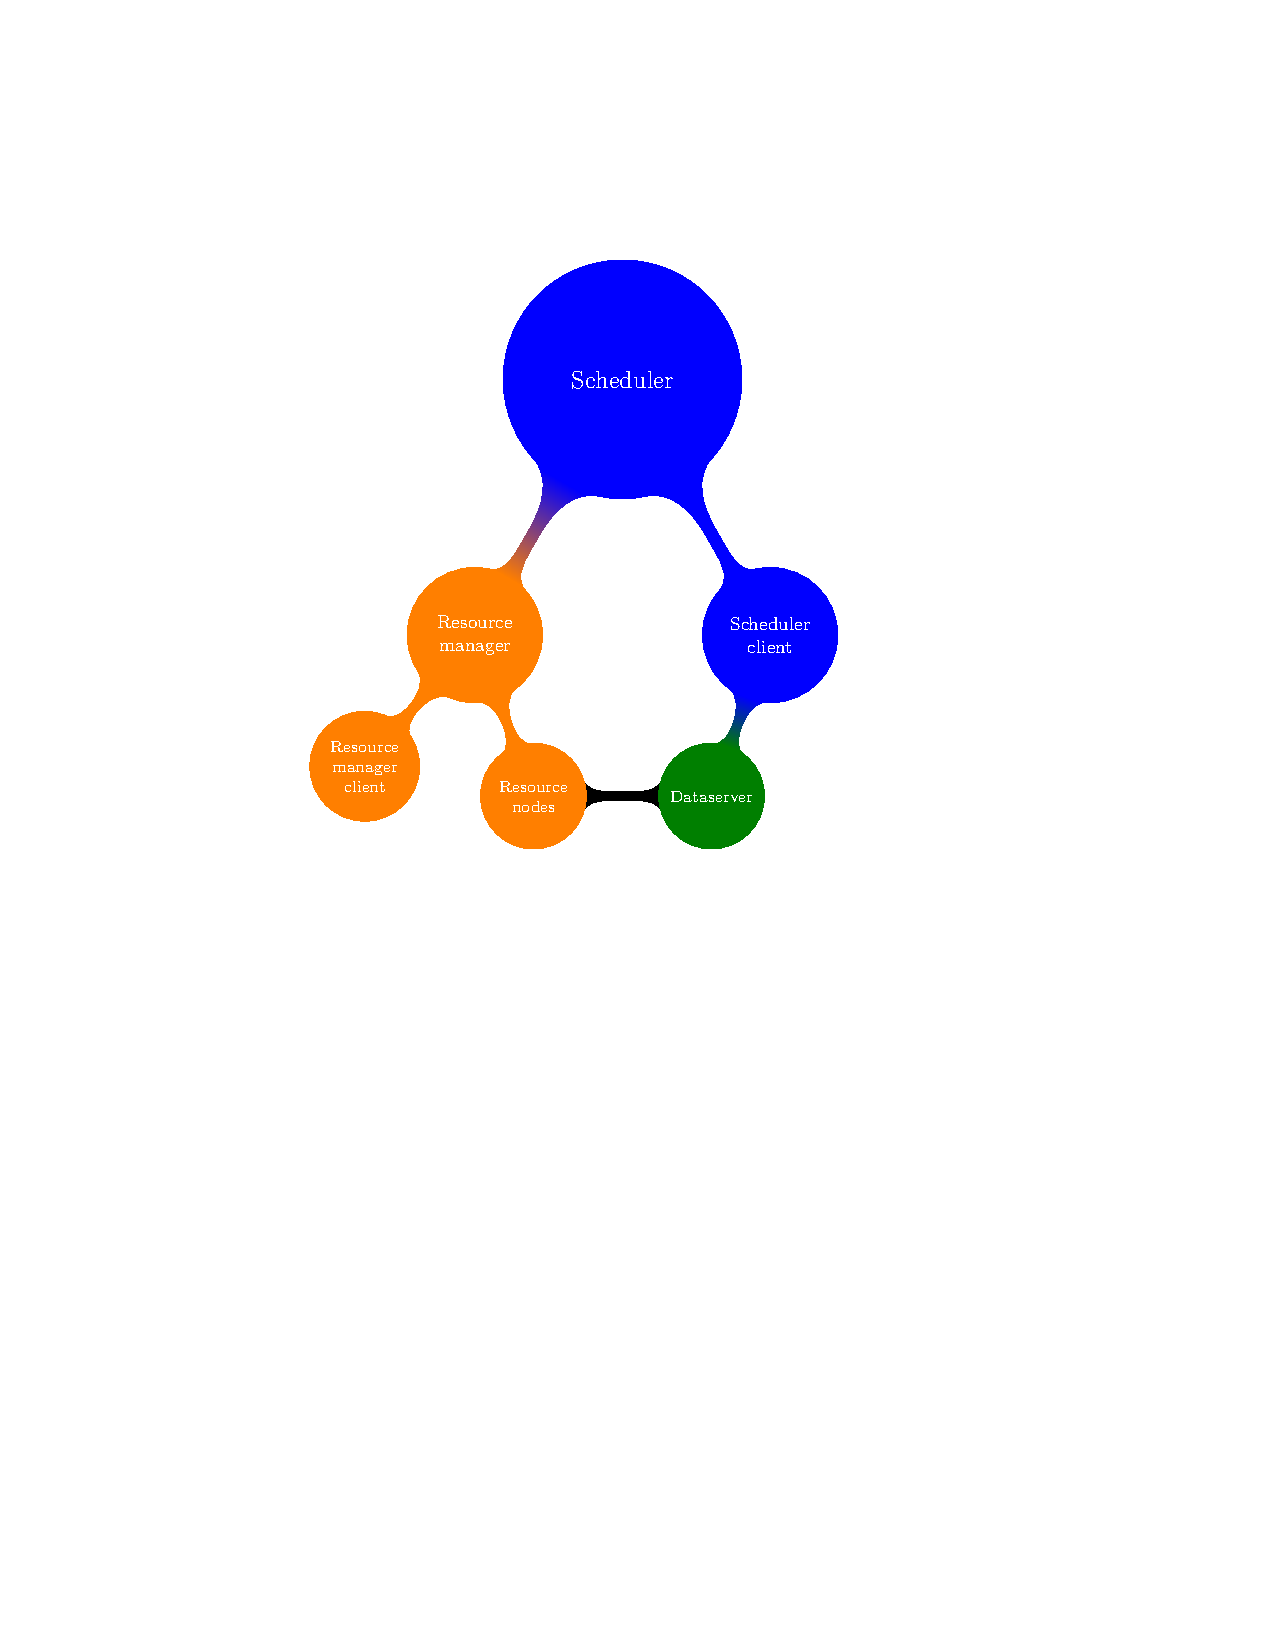
\includegraphics[trim=4cm 13cm 2cm 5cm,scale=0.48]{netmap_abs.pdf}
            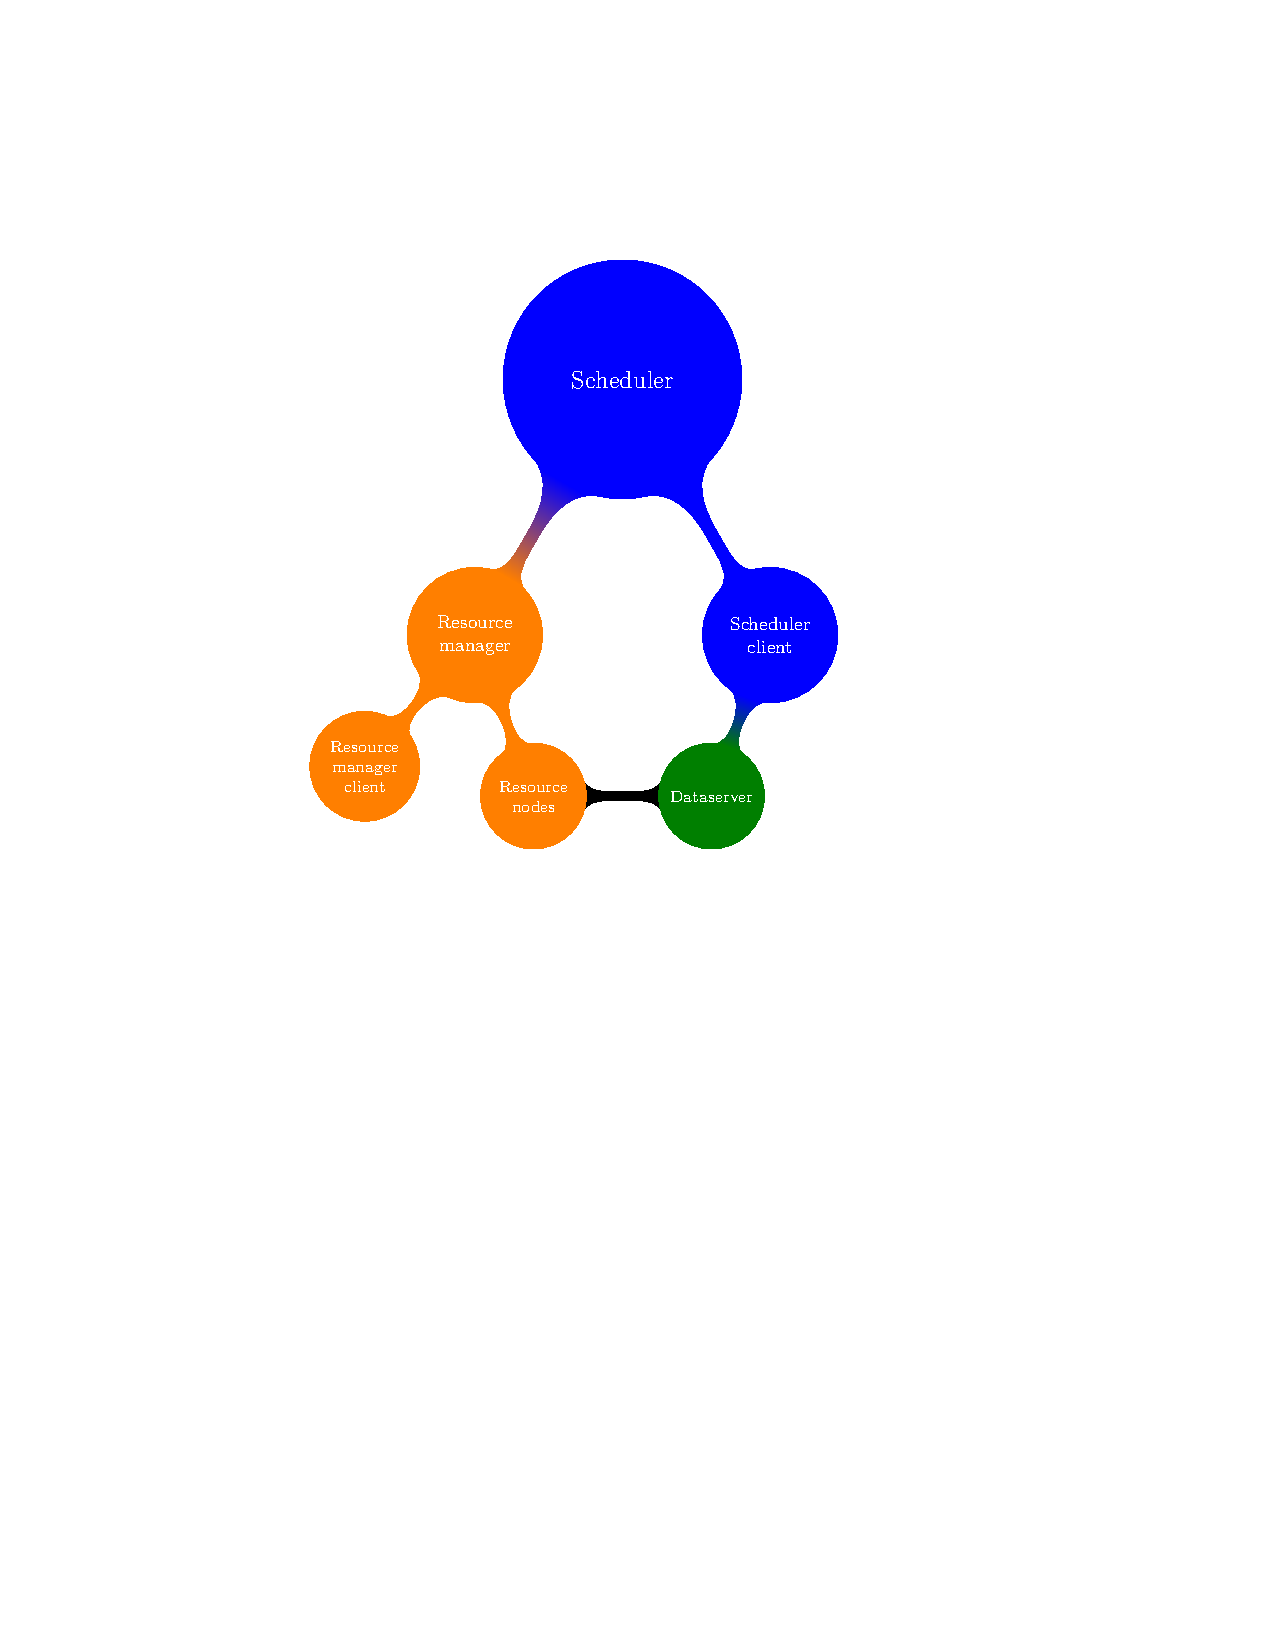
\includegraphics[trim=5.5cm 14.3cm 2cm 6.3cm,scale=0.69]{netmap_abs.pdf}
            %\caption{Communication dans Proactive}
        \end{figure}
	\end{column}
    \setbeamercolor{block title}{fg=white,bg=blue}   
    \setbeamercolor{block body}{fg=black,bg=blue!30}
	\begin{column}[r]{0.5\linewidth}
        \begin{block}{Scheduler}
            \begin{itemize}
            \item Affectation des calculs aux resource nodes
            \item Droits d'accès aux ressources 
            \item Intermédiaire entre le client et le resource manager
            \item Authentification des clients 
            \end{itemize}
        \end{block}
        \begin{block}{Scheduler client}
            \begin{itemize}
            \item Interface avec l'utilisateur
            \end{itemize}
        \end{block}
        
	\end{column}
	\end{columns}
    
\end{frame}

\begin{frame}{Dataserver}
	\begin{columns}
	\begin{column}[l]{0.5\linewidth}
        \begin{figure}
            %[!bh]
            \centering
            %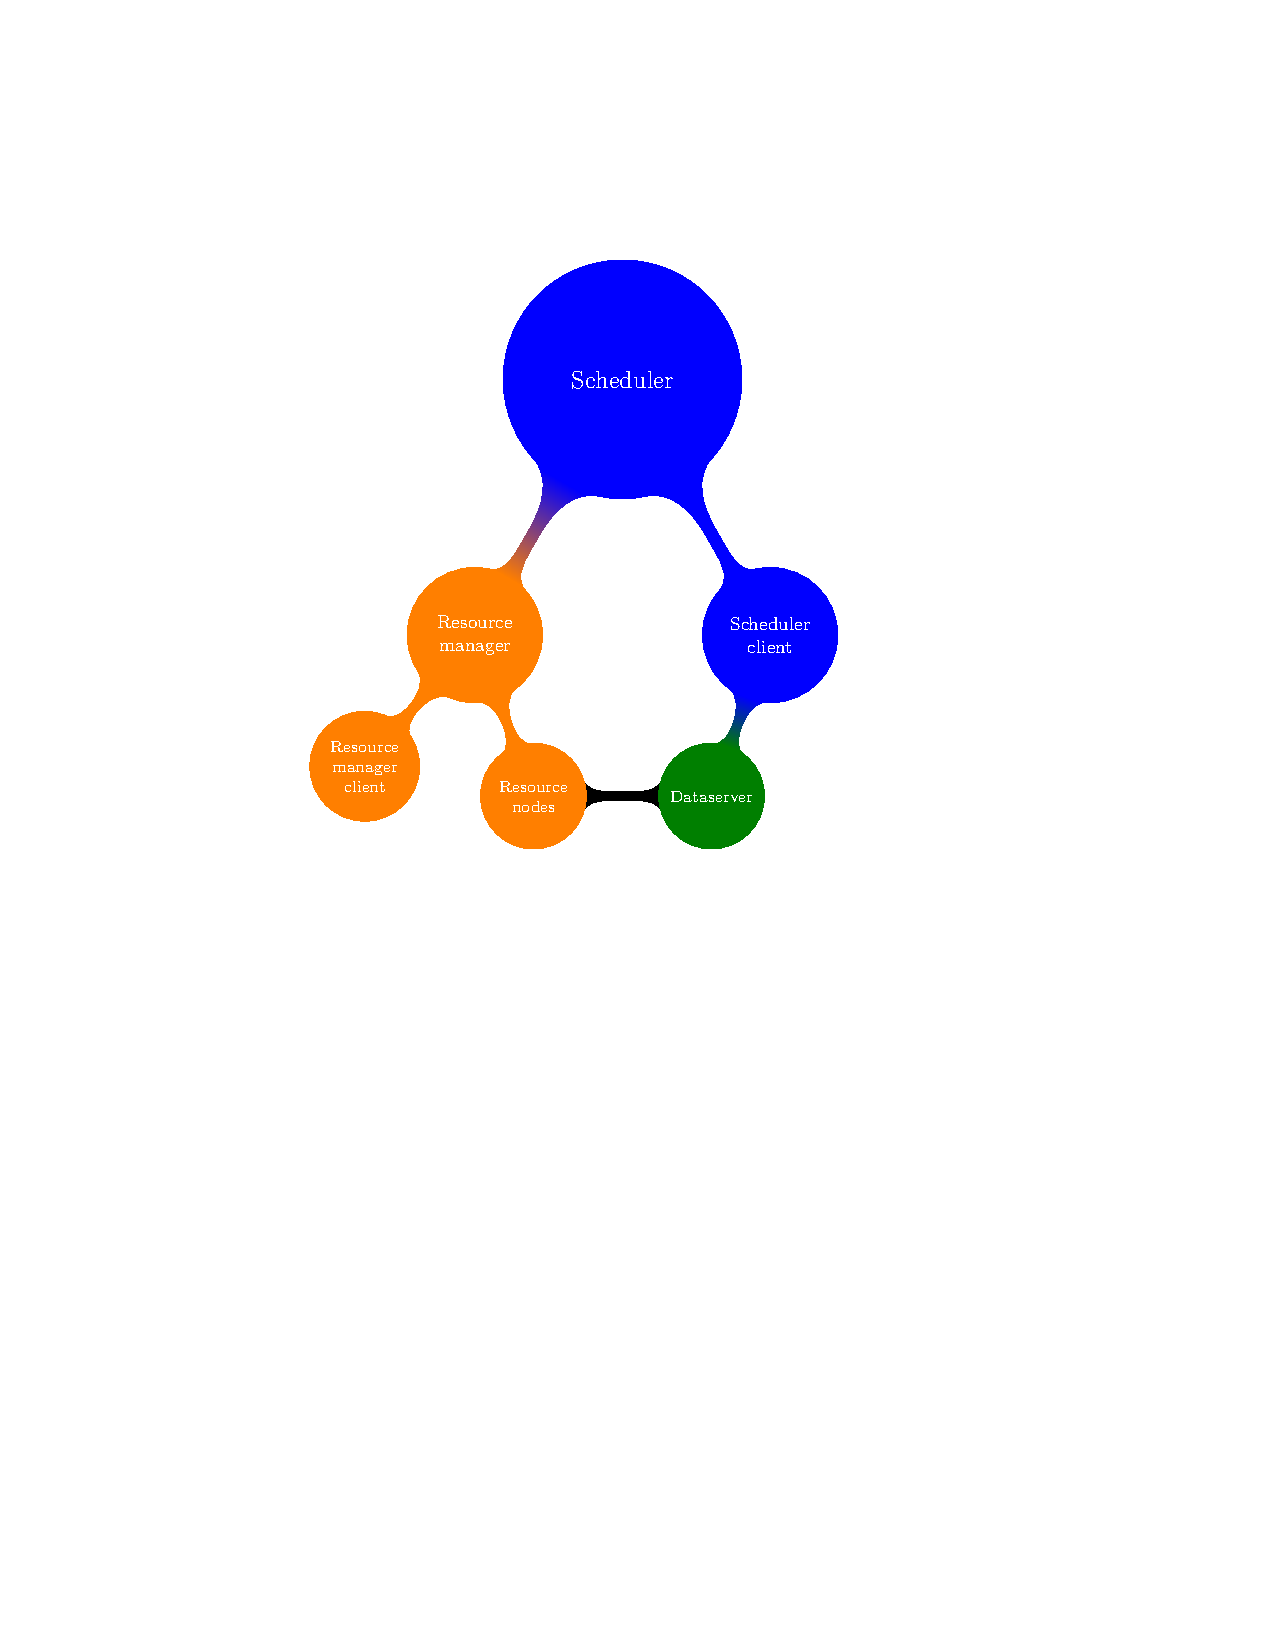
\includegraphics[trim=4cm 13cm 2cm 5cm,scale=0.48]{netmap_abs.pdf}
            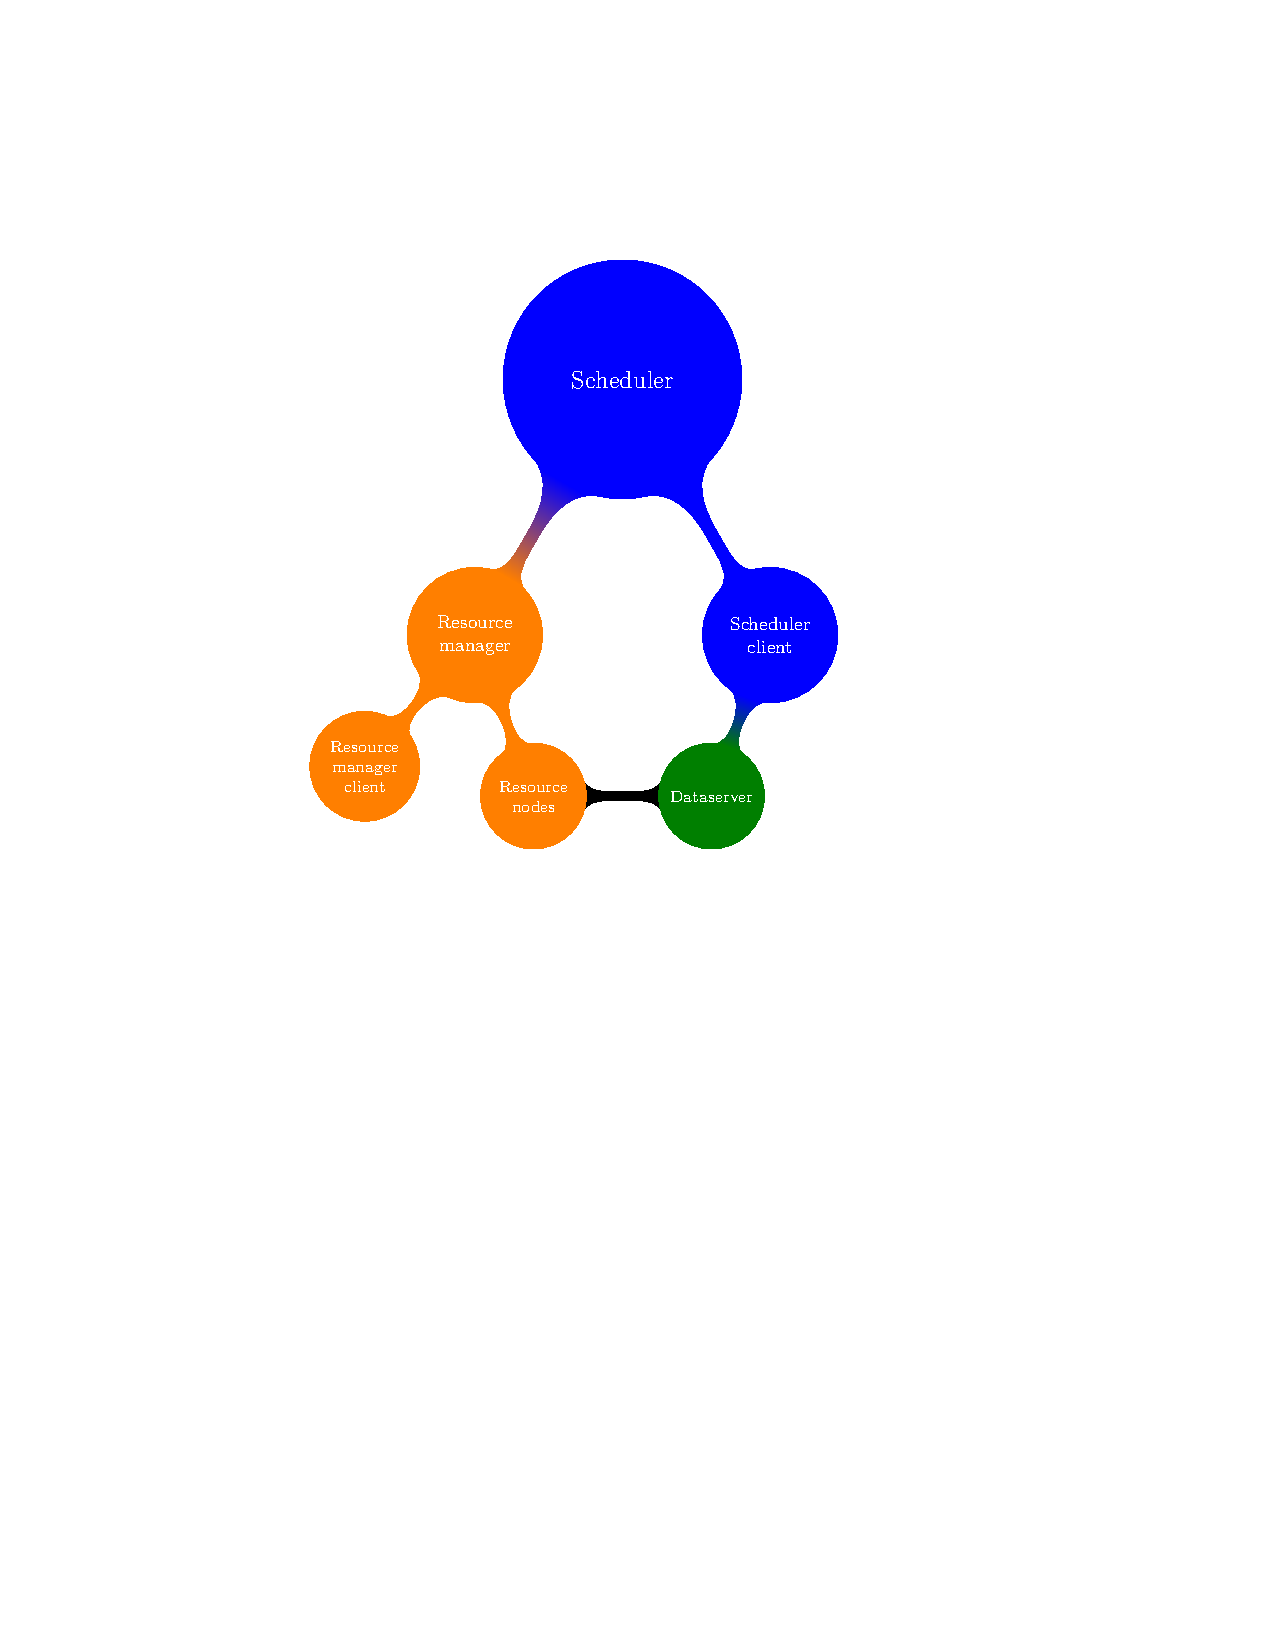
\includegraphics[trim=5.5cm 14.3cm 2cm 6.3cm,scale=0.69]{netmap_abs.pdf}
            %\caption{Communication dans Proactive}
        \end{figure}
	\end{column}
    \setbeamercolor{block title example}{fg=white,bg=green!50!black}   
    \setbeamercolor{block body example}{fg=black,bg=green!15}
	\begin{column}[r]{0.5\linewidth}
        \begin{exampleblock}{Dataserver}
            \begin{itemize}
                \item Crée un espace accessible en lecture et en écriture

             %Peut être lancé par un administrateur pour fournir un espace permanent commun à tous les utilisateurs (faisable au CBGP, petite taille)
             %peut être lancé par chaque client pour créer l'espace sur sa propre machine
             \item Permanent ou temporaire et commun ou personnel
             \item Espace partageable entre différents clients et calculs
             %Plusieurs client peuvent avoir accès au même espace
            \end{itemize}
            
        \end{exampleblock}
        
	\end{column}
	\end{columns}
    
\end{frame}
%\subsection{Architecture}
%
%\begin{frame}{Communication dans Proactive}
%    \begin{figure}
%        %[!bh]
%        \centering
%        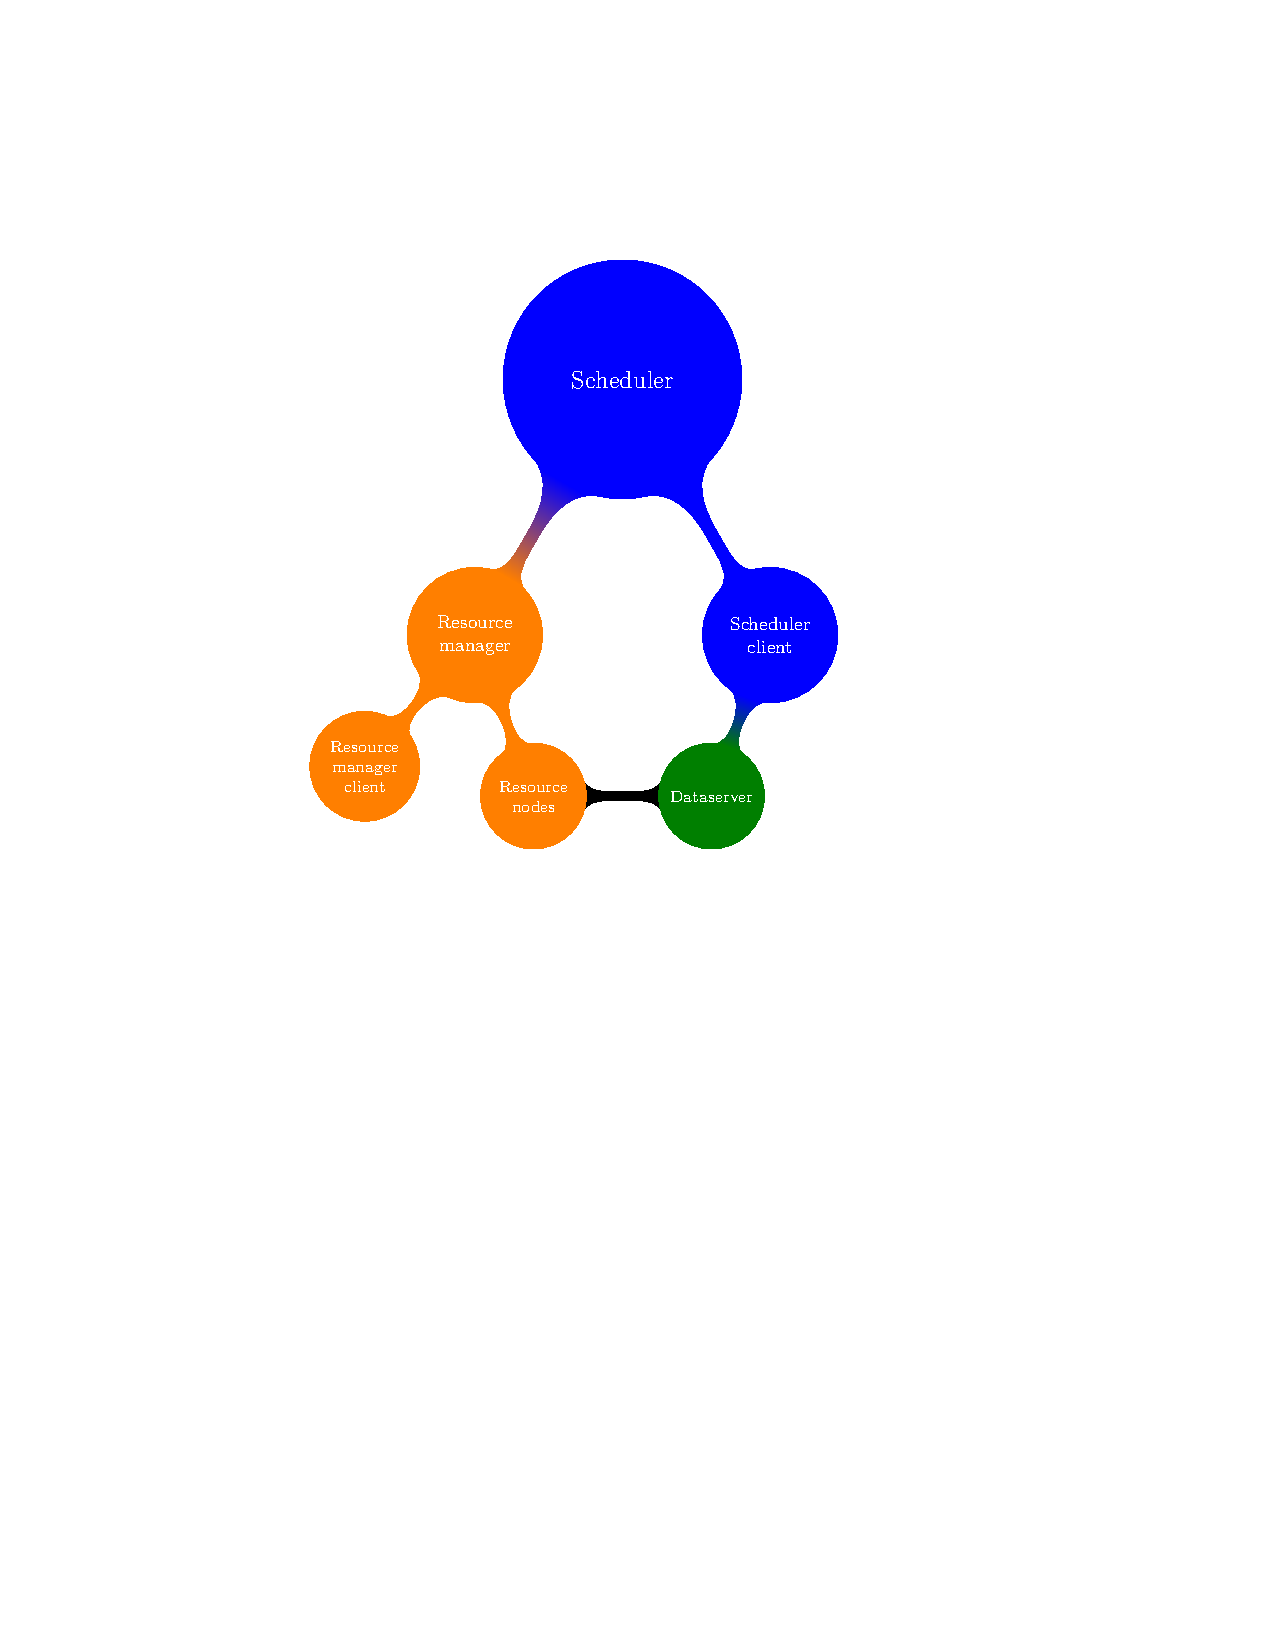
\includegraphics[trim=4cm 13cm 4cm 4cm,scale=0.62]{netmap_abs.pdf}
%        %\caption{Principe de communication dans le réseau Proactive}
%    \end{figure}
%    
%\end{frame}

\begin{frame}{Use case : soumission d'un calcul}
	\begin{columns}
	\begin{column}[l]{0.5\linewidth}
        \only<1>{\begin{figure}
            %[!bh]
            \centering
            %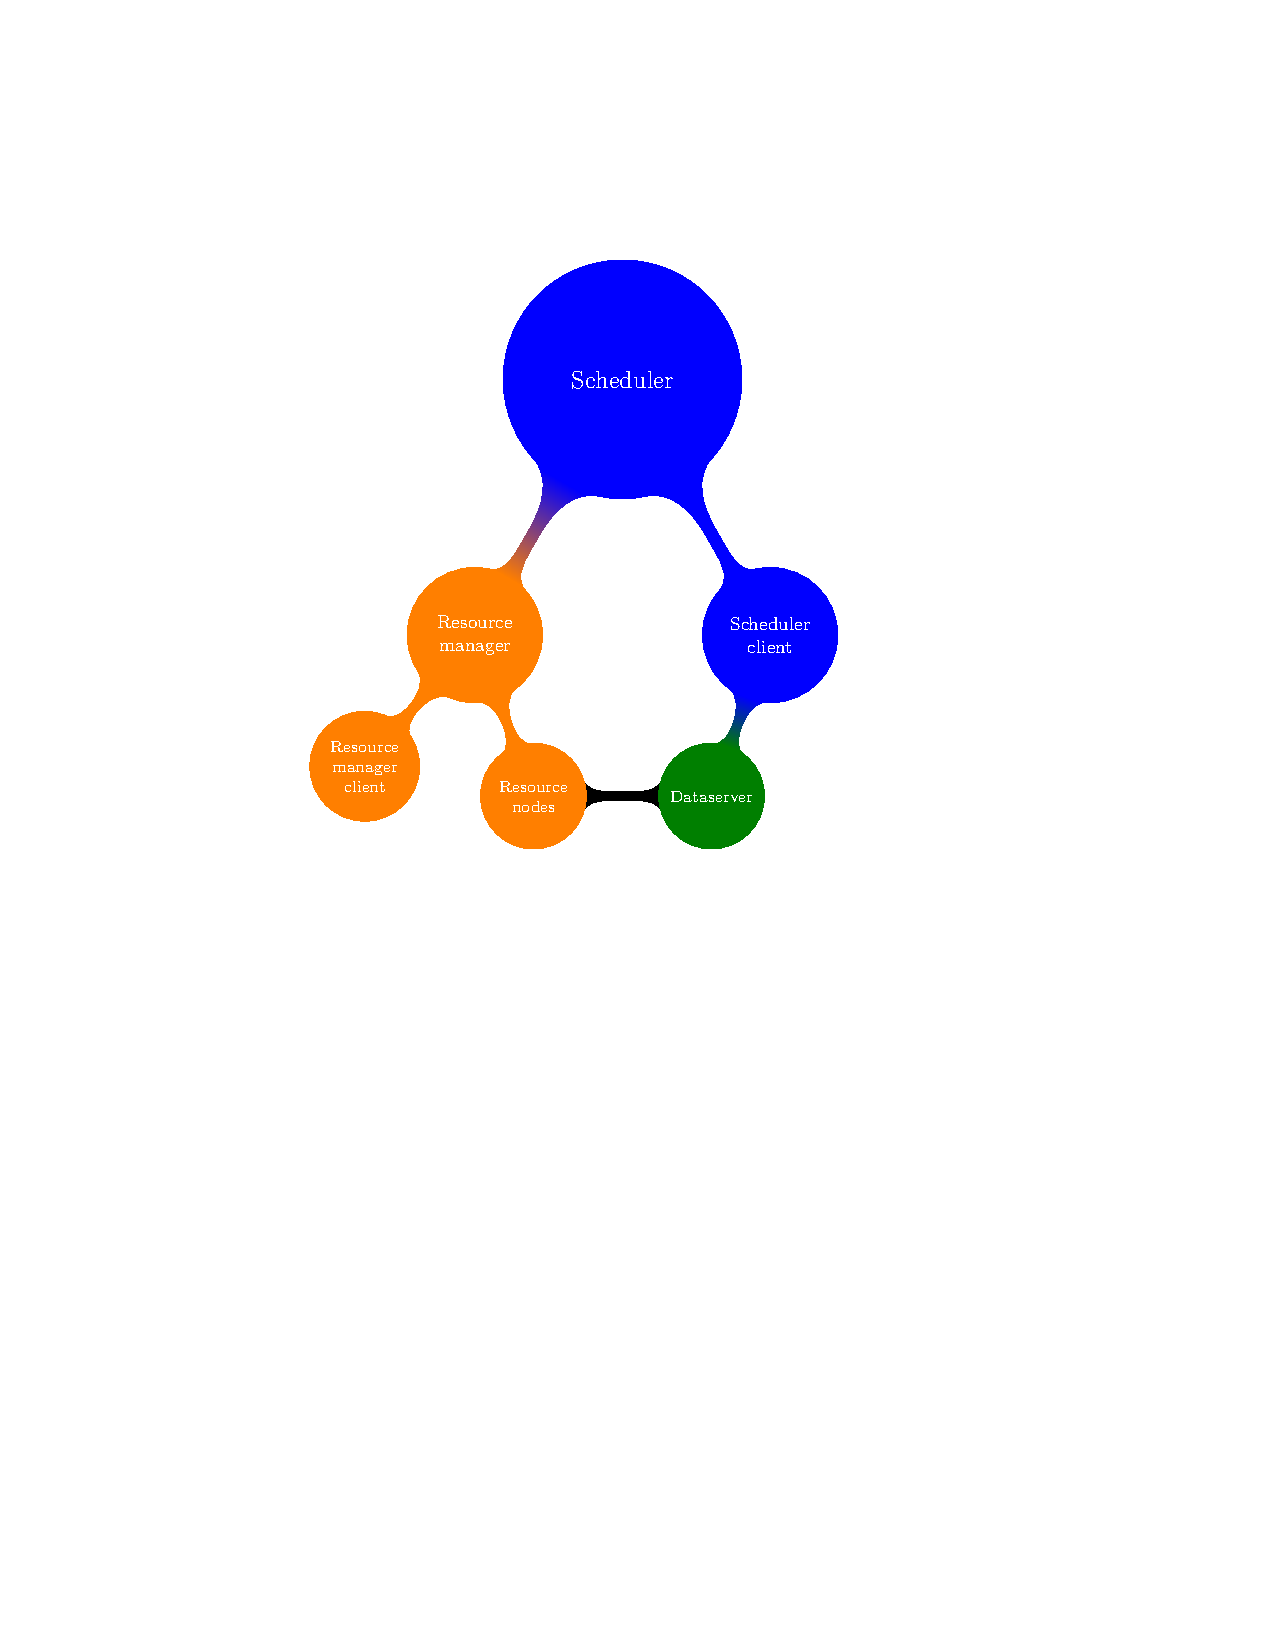
\includegraphics[trim=4cm 13cm 2cm 5cm,scale=0.48]{netmap_abs.pdf}
            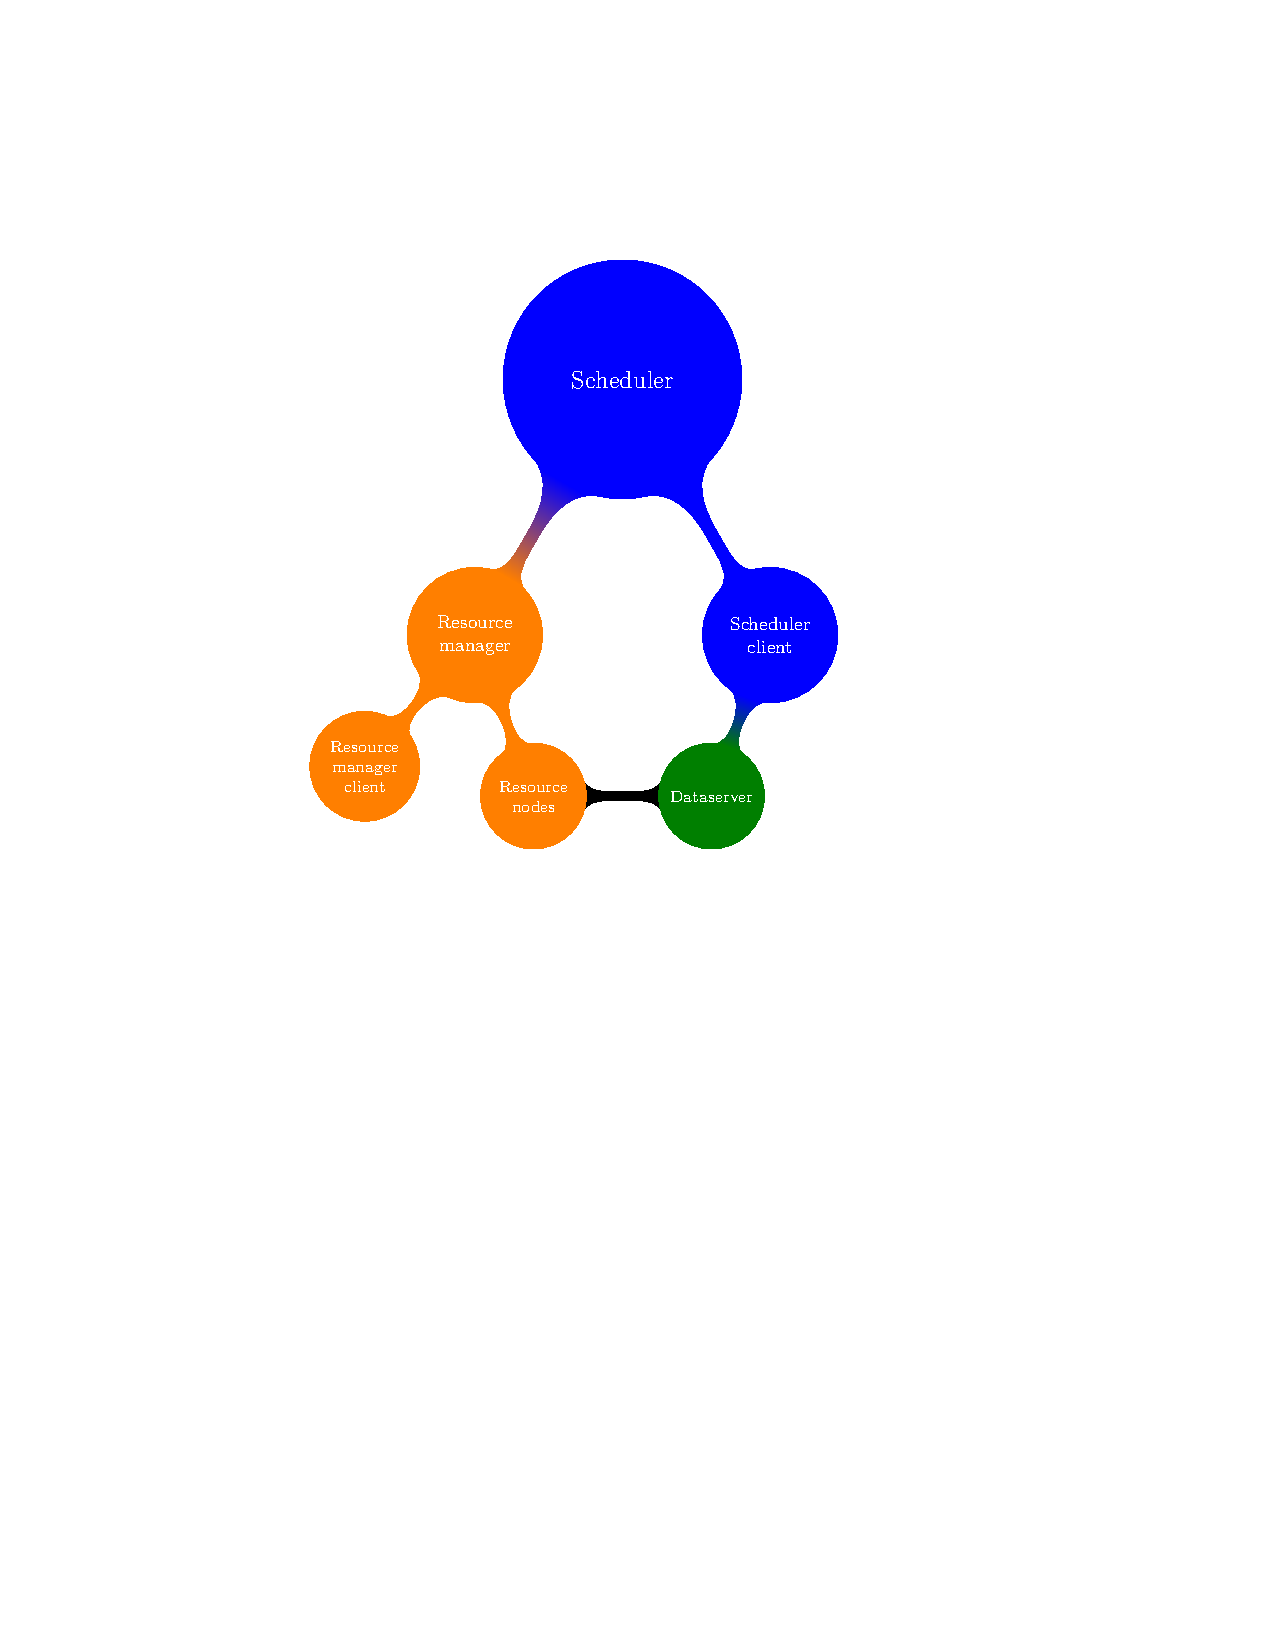
\includegraphics[trim=5.5cm 14.3cm 2cm 6.3cm,scale=0.69]{netmap_abs.pdf}
            %\caption{Communication dans Proactive}
        \end{figure}}
        \only<2>{\begin{figure}
            %[!bh]
            \centering
            %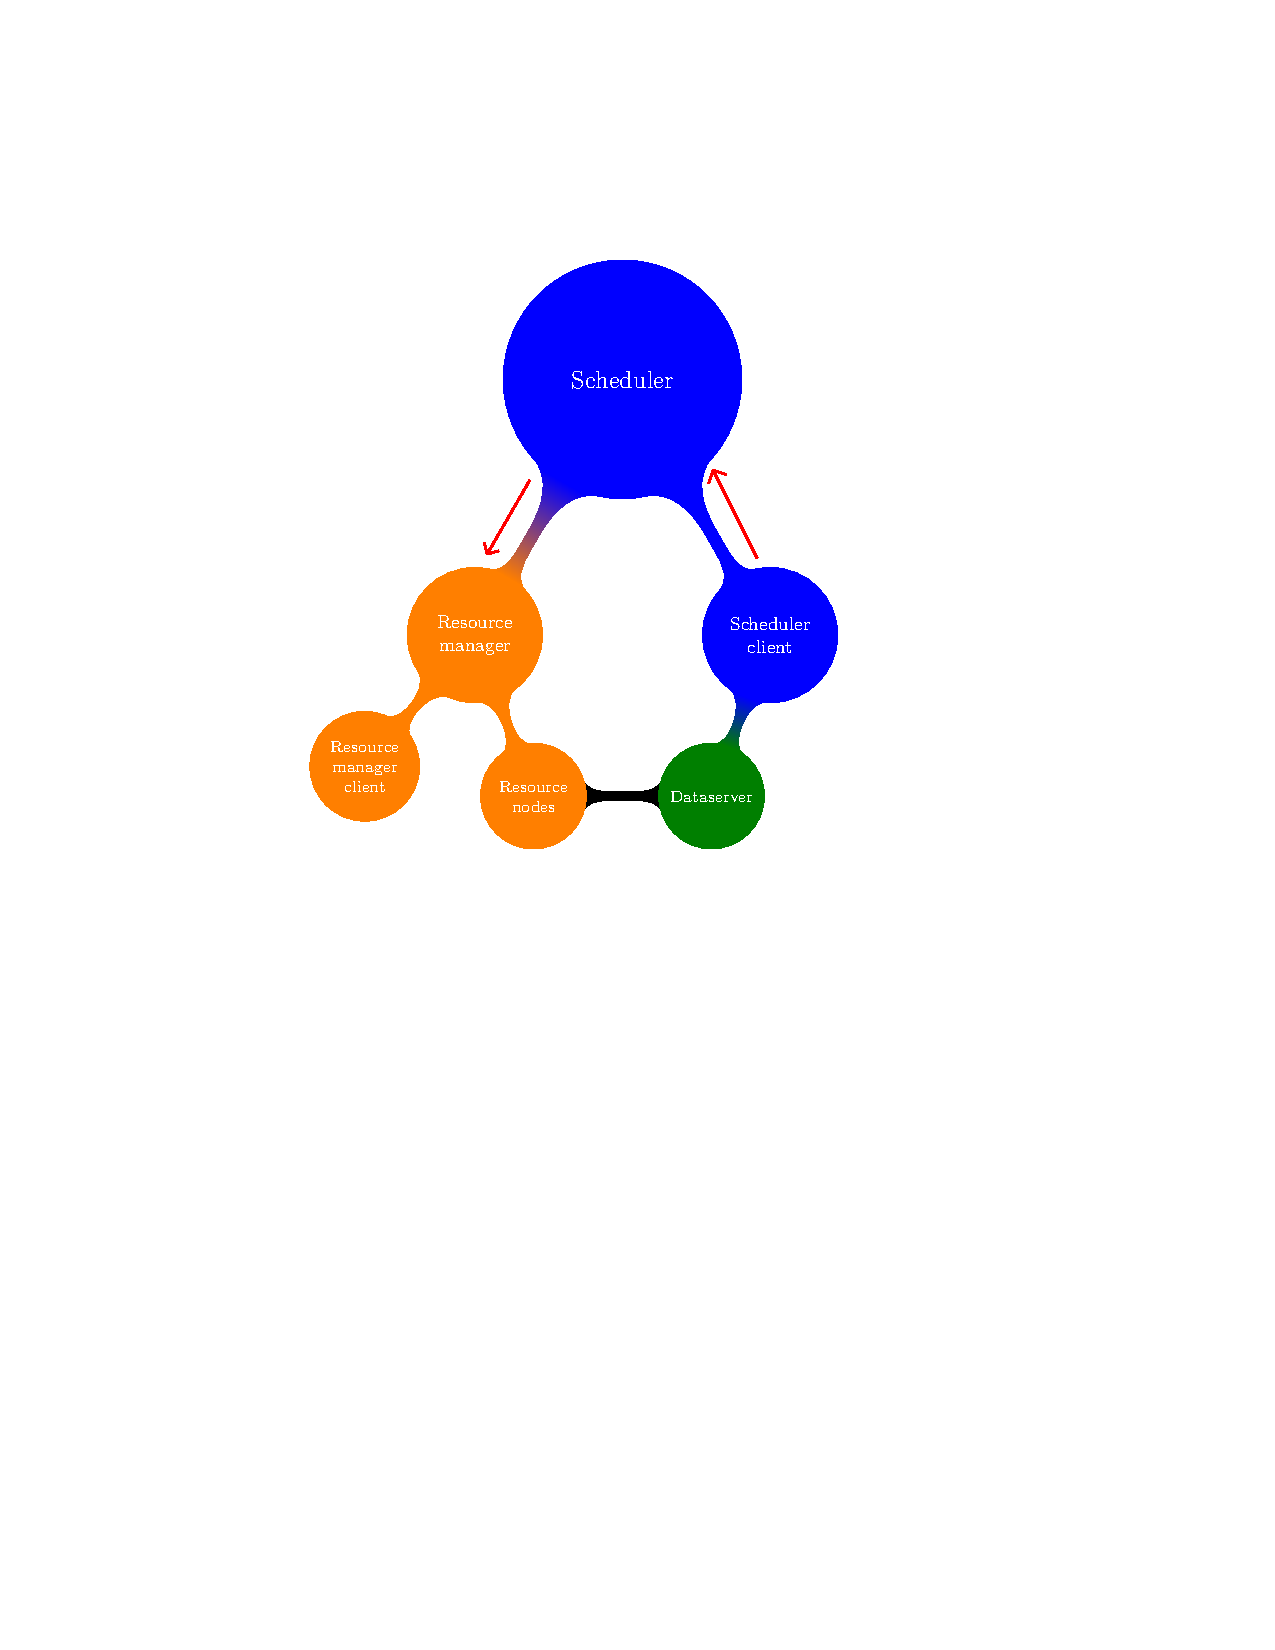
\includegraphics[trim=4cm 13cm 2cm 5cm,scale=0.48]{submit.pdf}
            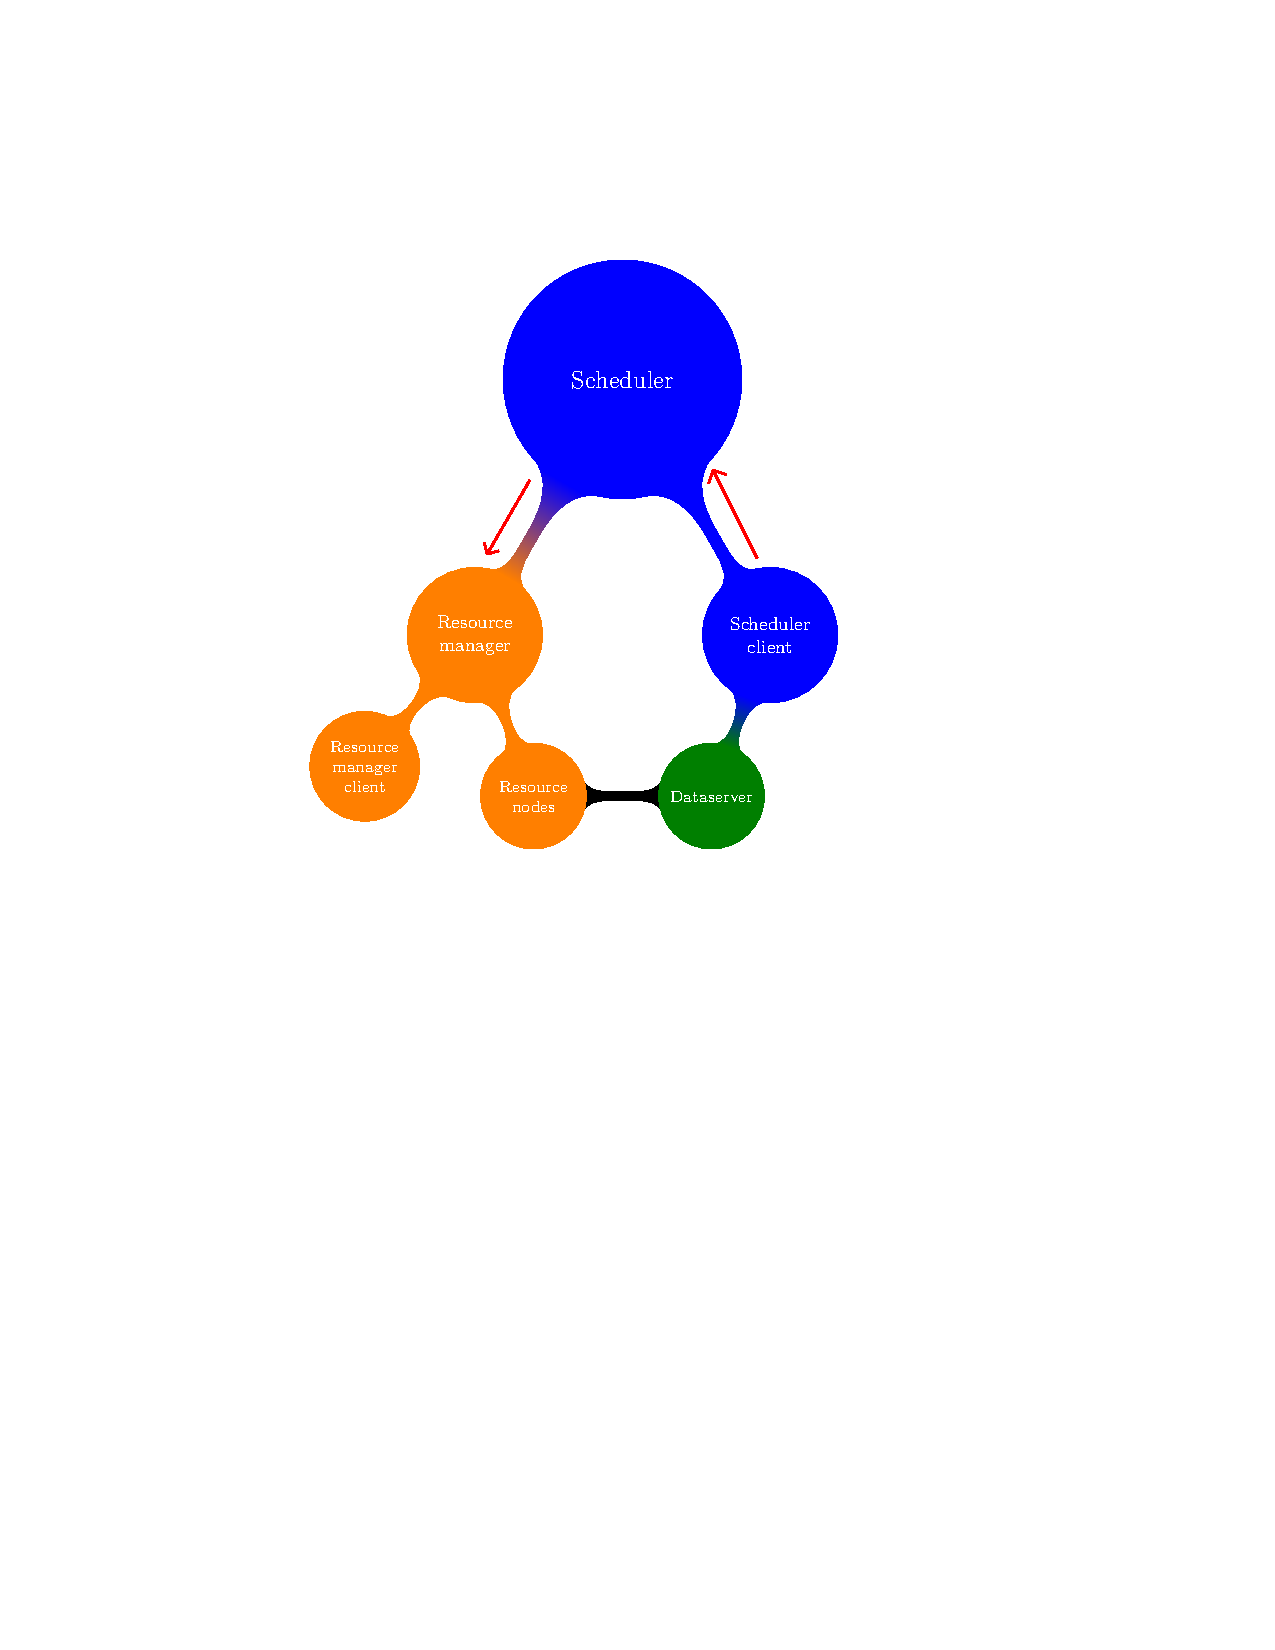
\includegraphics[trim=5.5cm 14.3cm 2cm 6.3cm,scale=0.69]{submit.pdf}
            %\caption{Communication dans Proactive}
        \end{figure}}
        \only<3>{\begin{figure}
            %[!bh]
            \centering
            %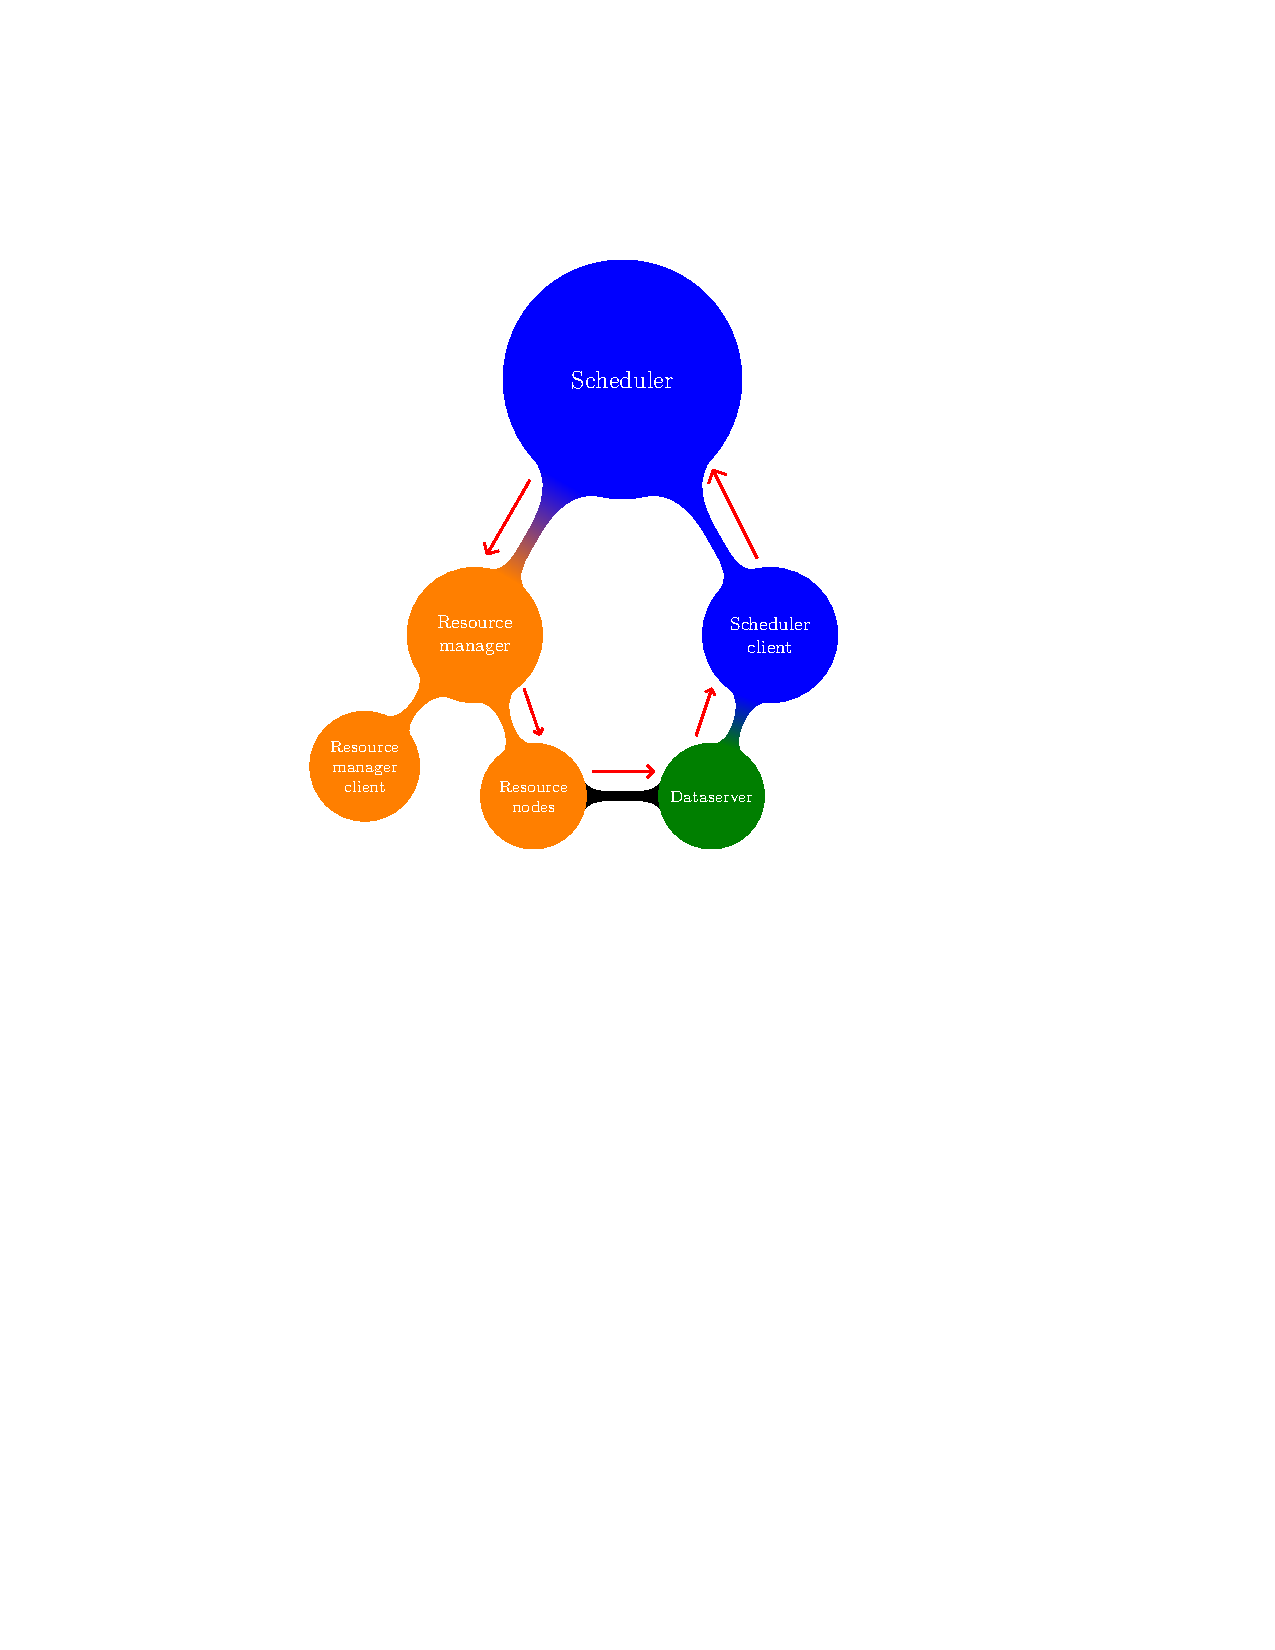
\includegraphics[trim=4cm 13cm 2cm 5cm,scale=0.48]{submit2.pdf}
            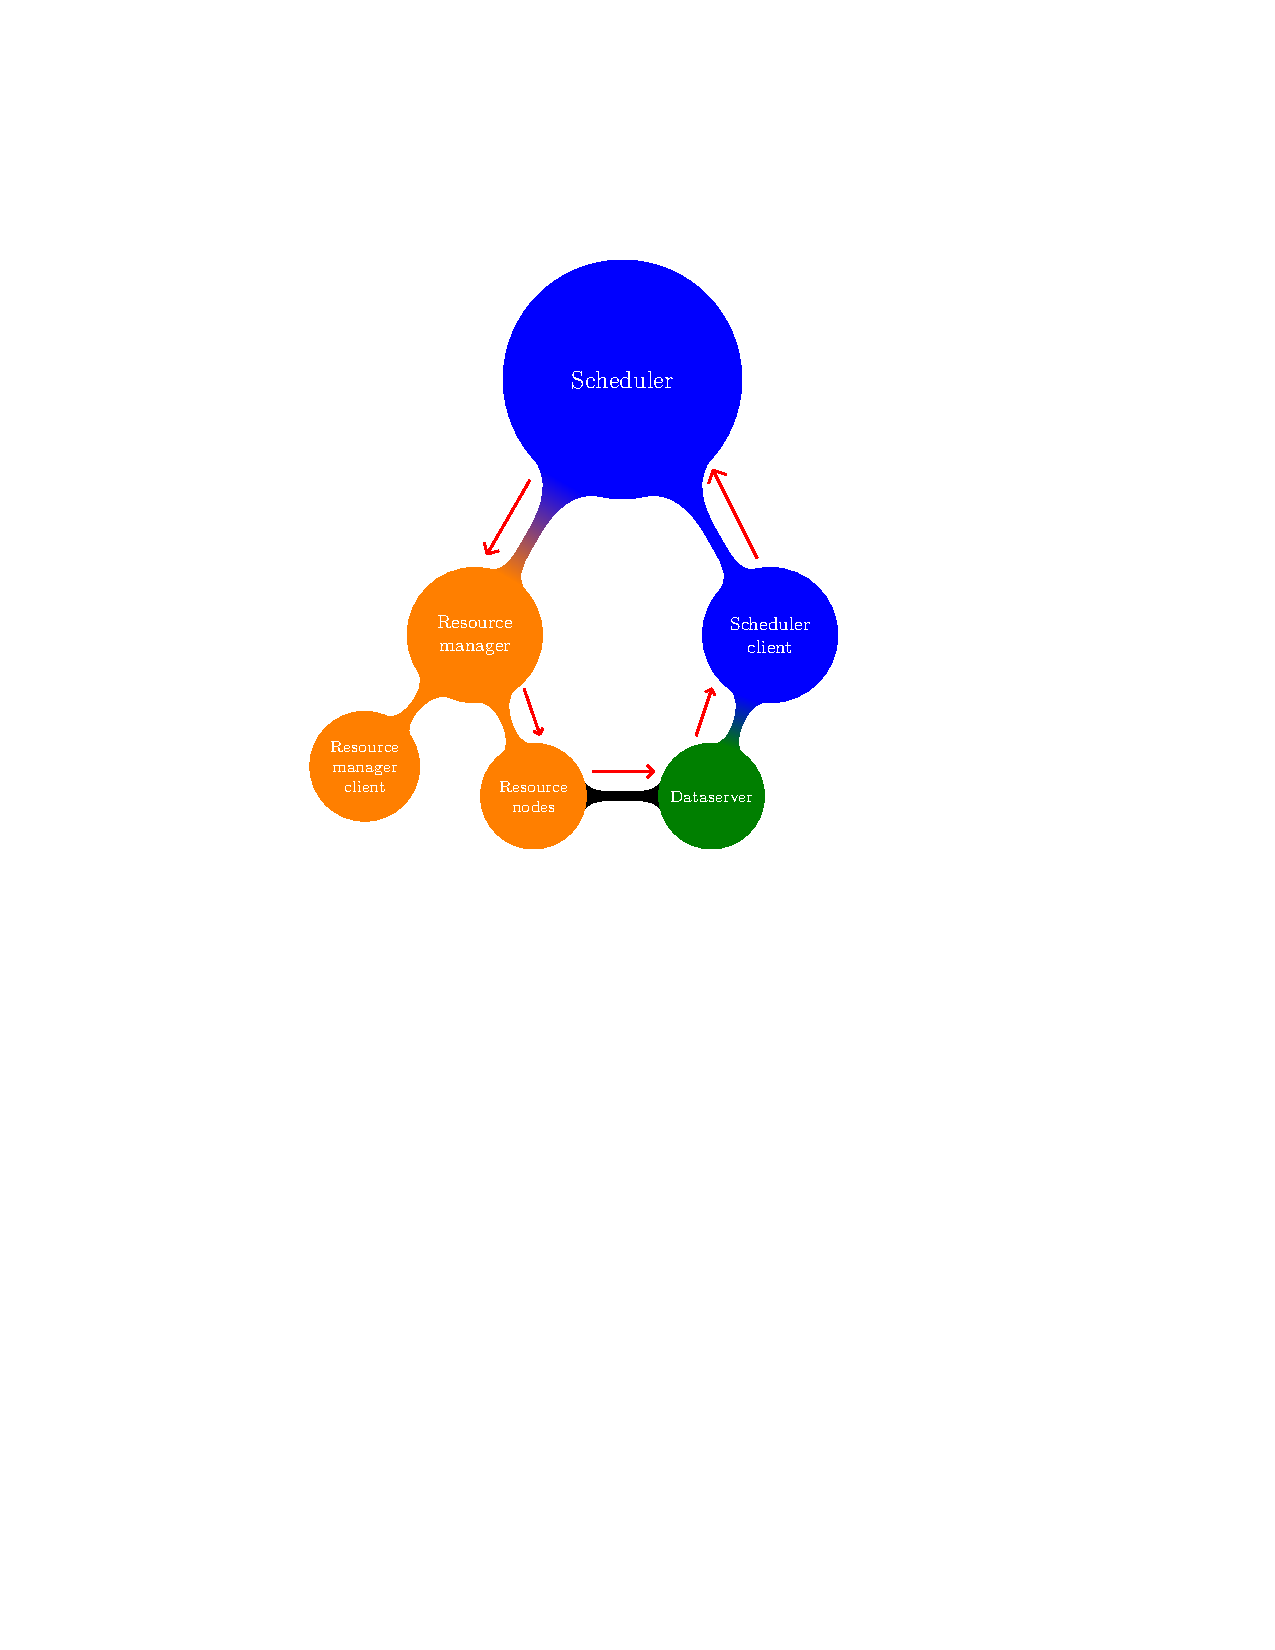
\includegraphics[trim=5.5cm 14.3cm 2cm 6.3cm,scale=0.69]{submit2.pdf}
            %\caption{Communication dans Proactive}
        \end{figure}}
	\end{column}
    \setbeamercolor{block title}{fg=white,bg=red!50!black}   
    \setbeamercolor{block body}{fg=black,bg=red!10}
	\begin{column}[r]{0.5\linewidth}
        \only<2-3>{
        \begin{block}{Soumission d'un calcul}
            \begin{itemize}
            \item<2-> Transmission au scheduler
            \item<2-> Transmission au resource manager
            \item<3-> Affectation aux nodes
            \item<3-> Transmission des résultats
            \end{itemize}
        \end{block}
        }
        
	\end{column}
	\end{columns}
    
\end{frame}

\subsection{Outils graphiques}
\begin{frame}
	\tableofcontents[currentsubsection]
\end{frame}
\begin{frame}{Scheduler client}
    % interessant pour la partie job submission et job results
    \begin{figure}
        %[!bh]
        \centering
        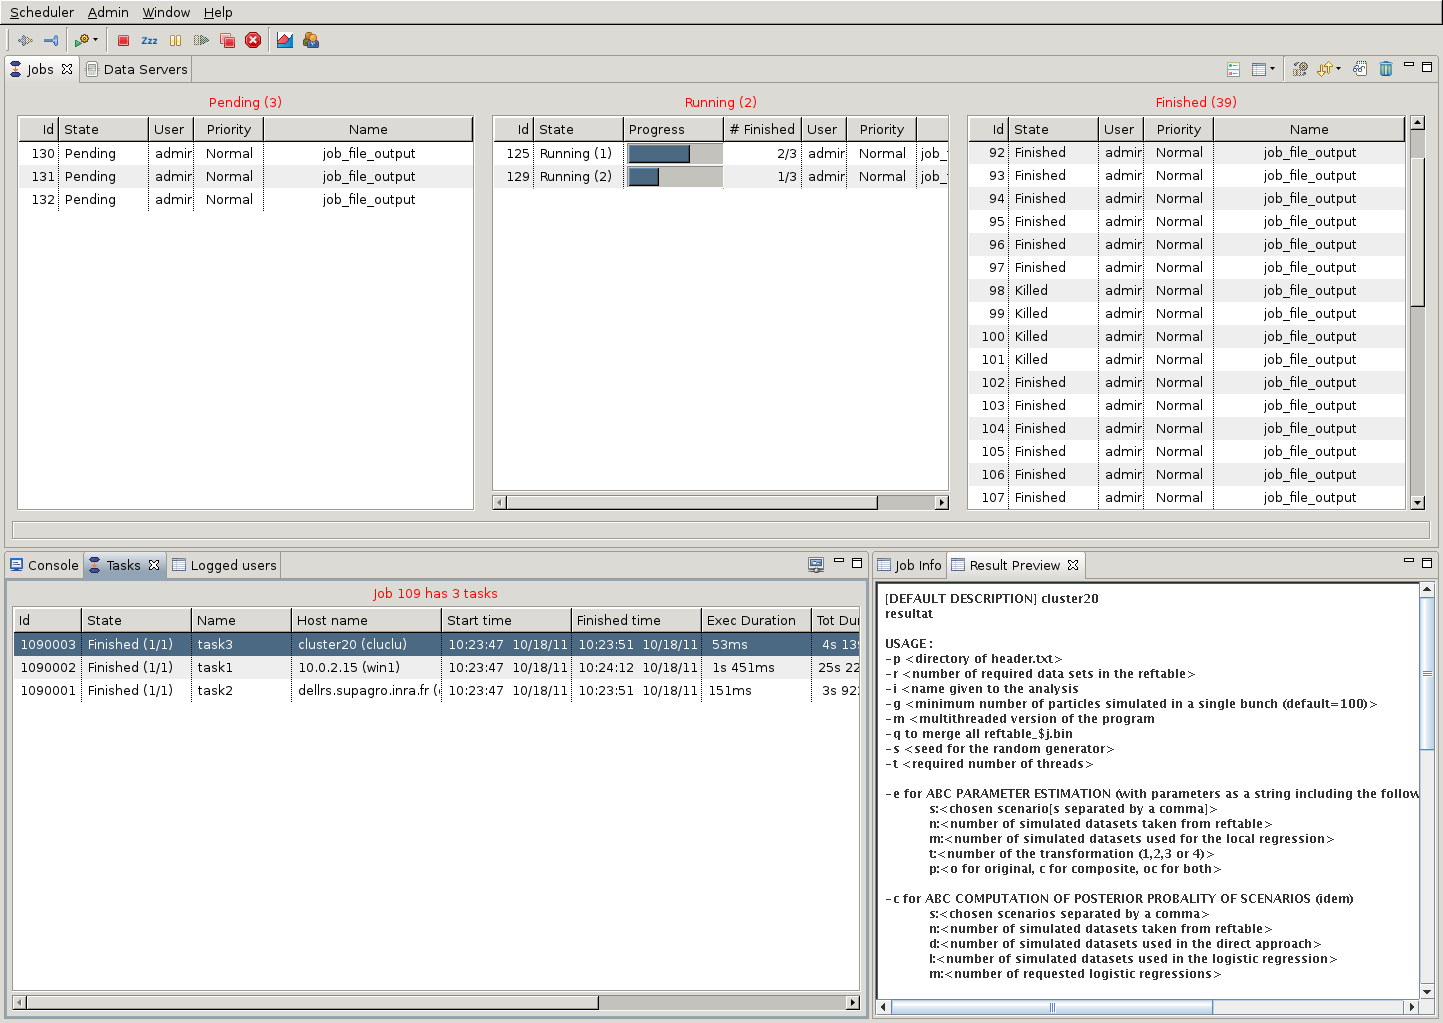
\includegraphics[scale=0.18]{sc_sched.png}
        %\caption{Principe de communication dans le réseau Proactive}
    \end{figure}
\end{frame}
\begin{frame}{Resource manager client}
    % interessant pour la partie monitoring
    \begin{figure}
        %[!bh]
        \centering
        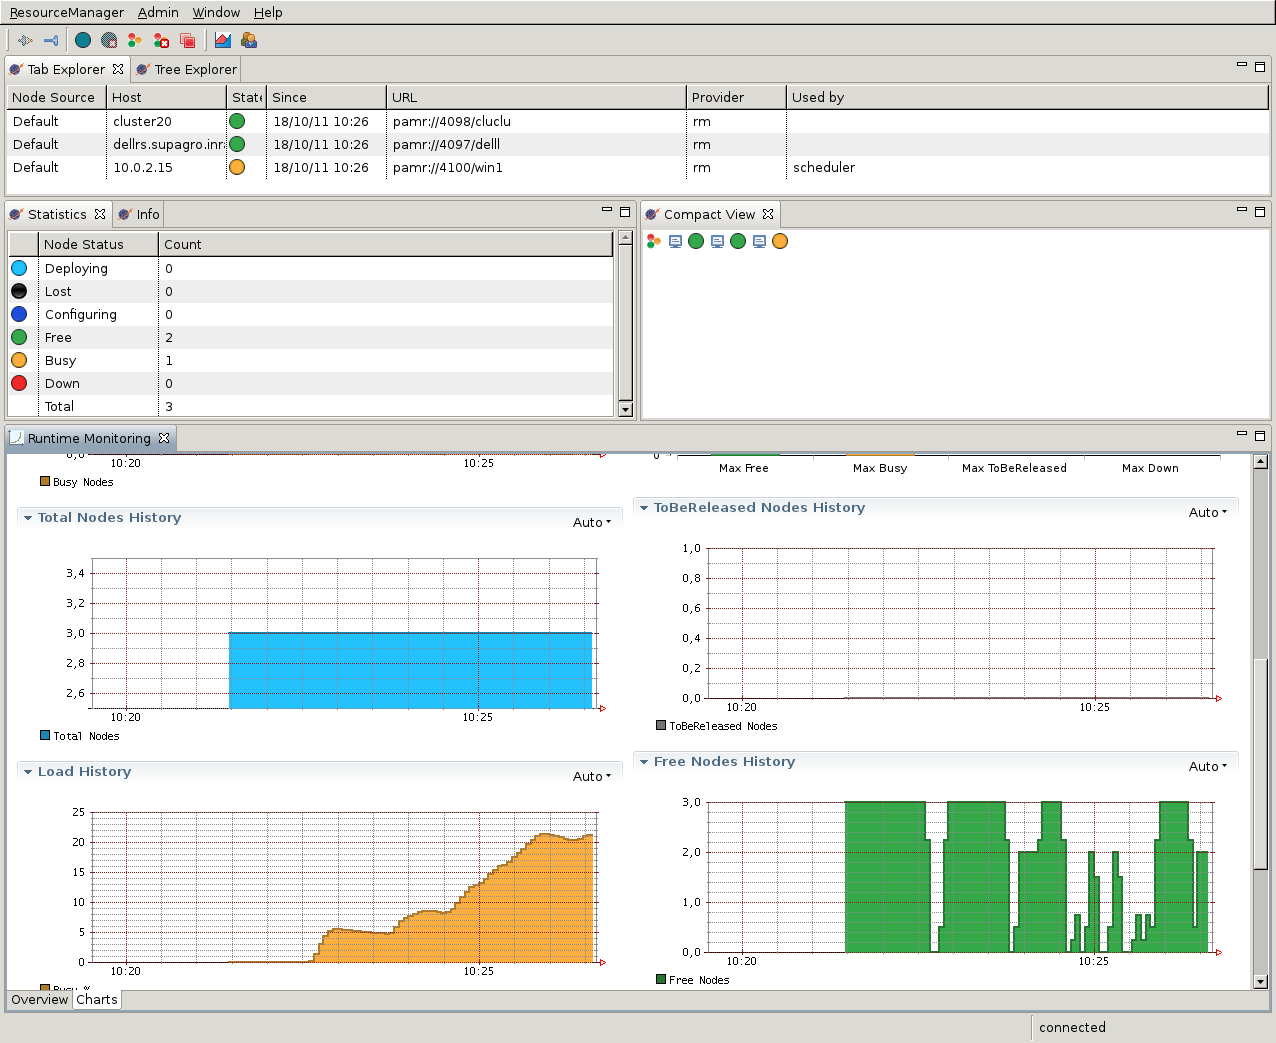
\includegraphics[scale=0.18]{sc_rmc.png}
        %\caption{Principe de communication dans le réseau Proactive}
    \end{figure}
\end{frame}


\subsection{Définition d'un calcul}
\begin{frame}
	\tableofcontents[currentsubsection]
\end{frame}
\begin{frame}
    \setbeamercolor{block title}{fg=white,bg=red!50!black}   
    \setbeamercolor{block body}{fg=black,bg=red!10}
    \vspace{-0.15cm}
        \begin{block}{Qu'est-ce qu'un calcul ? (Job)}<1->
        % en java, par xml, ou par liste de commandes
            \begin{itemize}
                \item Un identifiant
                \item Un serveur de données
                \item Une liste d'opérations à effectuer (tasks)%option dependances, retry..
            \end{itemize}
        \end{block}
        \begin{block}{Quels sont les types de task ?}<2->
        % en java, par xml, ou par liste de commandes
            \begin{itemize}
                \item Natif : Lance un script/binaire qui doit être compatible avec le resource node
                \item Java : Transport et lancement d'un exécutable Java
            \end{itemize}
        \end{block}
        \begin{block}{Options}<3->
            \begin{itemize}
                \item Intégration d'options similaires à celles de SGE
                \item Job : Priority, inputSpace, outputSpace, variables
                \item Task : restartTaskOnError, inputFiles, outputFiles, \textbf{depends}, selectionScript
            \end{itemize}
        \end{block}
\end{frame}
\begin{frame}{Types de définition}
    \setbeamercolor{block title}{fg=white,bg=red!50!black}   
    \setbeamercolor{block body}{fg=black,bg=red!10}
    \begin{block}{Trois manières de définir un job}
        \begin{itemize}
            \item Liste de commandes
            \item XML
            \item Java
        \end{itemize}
    \end{block}
    
\end{frame}

\begin{frame}{Avec une liste de commandes natives}
    \setbeamercolor{block title}{fg=white,bg=red!50!black}   
    \setbeamercolor{block body}{fg=black,bg=red!10}
	\begin{columns}
	\begin{column}[l]{0.4\linewidth}
        \begin{block}{liste}
            \begin{itemize}
                \item Jobs natifs uniquement (possibilité de sélection des nodes)
                \item Liste de commandes qui seront exécutées directement sur un noeud de calcul
                \item Gestion basique
            \end{itemize}
        \end{block}
	\end{column}
	\begin{column}[r]{0.6\linewidth}
        /path/to/script\_1.sh arg1 arg2\newline
        /path/to/script\_2.sh arg3 arg4\newline
        /path/to/script\_3.sh arg5 arg6\newline
	\end{column}
	\end{columns}
    
\end{frame}
\begin{frame}{En XML}
    \setbeamercolor{block title}{fg=white,bg=red!50!black}   
    \setbeamercolor{block body}{fg=black,bg=red!10}
	\begin{columns}
	\begin{column}[l]{0.4\linewidth}
        \begin{block}{Définition par XML}
            \begin{itemize}
                \item Jobs natifs ou Java
                \item Fichier XML qui spécifie chaque paramètre
                \item Plus simple mais moins complète que Java
            \end{itemize}
        \end{block}
	\end{column}
	\begin{column}[r]{0.6\linewidth}
        \vspace{-1cm}
        \begin{figure}
            %[!bh]
            \centering
            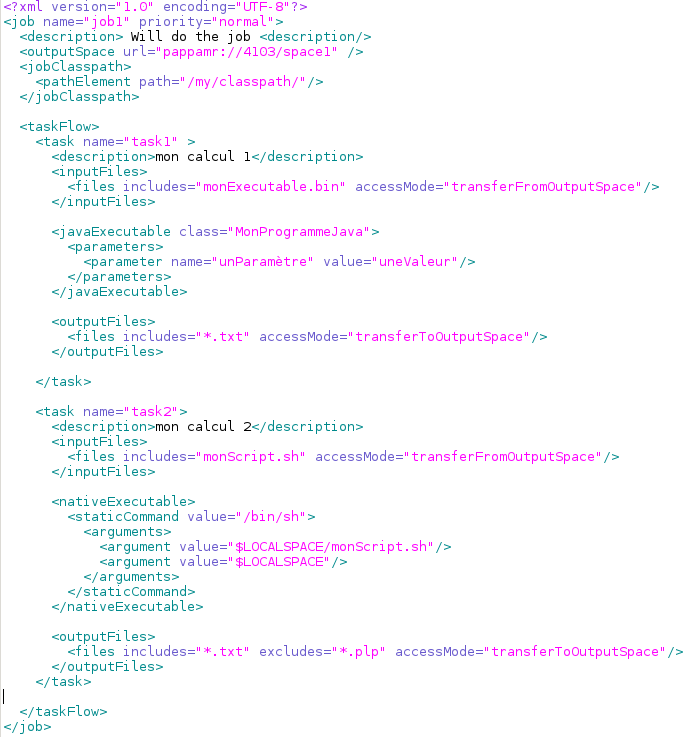
\includegraphics[scale=0.27]{jobxml.png}
            %\caption{Communication dans Proactive}
        \end{figure}
	\end{column}
	\end{columns}
    
\end{frame}
\begin{frame}{En Java}
    \setbeamercolor{block title}{fg=white,bg=red!50!black}   
    \setbeamercolor{block body}{fg=black,bg=red!10}
	\begin{columns}
	\begin{column}[l]{0.4\linewidth}
        \begin{block}{Définition dans un programme en Java}
            \begin{itemize}
                \item Jobs natifs ou Java
                \item Directement dans un programme en Java qui se connecte au scheduler
                \item Gestion fine
            \end{itemize}
        \end{block}
	\end{column}
	\begin{column}[r]{0.6\linewidth}
        \vspace{-1cm}
        \begin{figure}
            %[!bh]
            \centering
            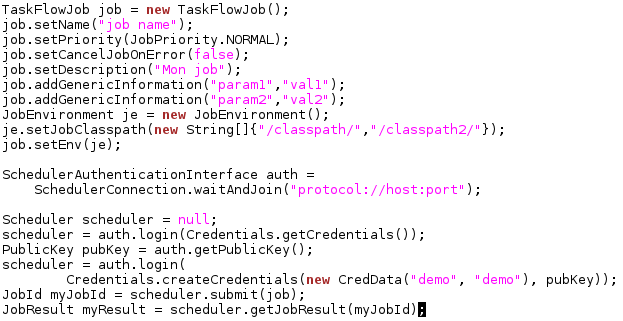
\includegraphics[scale=0.32]{jobjava.png}
            %\caption{Communication dans Proactive}
        \end{figure}
	\end{column}
	\end{columns}
    
\end{frame}


\section[Applications]{Applications possibles}
\begin{frame}
	\tableofcontents[currentsection]
\end{frame}
\subsection{Intégration avec un cluster}
\begin{frame}{Intégration des ressources d'un cluster existant}
    \setbeamercolor{block title}{fg=black,bg=violet}   
    \setbeamercolor{block body}{fg=black,bg=violet!10}
    \begin{block}{Protocoles}
    \begin{itemize}
        \item PBS (SGE, Torque \ldots)
        \item LSF
        \item SSH  
    \end{itemize}
        
    \end{block}
        \begin{figure}
            %[!bh]
            \centering
            \includegraphics[trim=1cm 14cm 2cm 4.6cm,scale=0.55]{res1.pdf}
            %\caption{}
        \end{figure}
\end{frame}
\subsection{Utilisation de ressources individuelles}
\begin{frame}
	\tableofcontents[currentsubsection]
\end{frame}
\begin{frame}{Les postes de travail}
    \setbeamercolor{block title}{fg=black,bg=red!65!black}   
    \setbeamercolor{block body}{fg=black,bg=red!10}
    \begin{block}{Déployer manuellement des resource nodes}
    Avec le programme des noeuds de calcul
        
    \end{block}
    \begin{block}{PA-Agent}
    Programme d'automatisation de la mise à disposition des ressources
        
    \end{block}
    \vspace{0.2cm}
        \begin{figure}
            %[!bh]
            \centering
            \includegraphics[trim=4cm 13cm 2cm 5.2cm,scale=0.55]{res2.pdf}
            %\caption{}
        \end{figure}
\end{frame}
\subsection{Cloud}
\begin{frame}
	\tableofcontents[currentsubsection]
\end{frame}
\begin{frame}{Utiliser les ressources d'un cloud}
    \setbeamercolor{block title}{fg=black,bg=orange}   
    \setbeamercolor{block body}{fg=black,bg=orange!10}
    \vspace{-0.2cm}
    \only<1>{\begin{block}{Quels types de cloud ?}
        \begin{itemize}
            \item Amazon Elastic Compute Cloud (EC2)
            \item Windows High Performance Computing (HPC)
        \end{itemize}
    \end{block}}

    \only<2>{\begin{block}{Comment ?}
      %  Machine virtuelle dupliquée sur les noeuds du cloud qui lance 
     %On utilise la ressource dont on a besoin (pas plus pas moins) et seulement quand on en a besoin

     \begin{itemize}
         \item Déploiement par machines virtuelles
         \item Déploiement par outil interne 
     \end{itemize}
        
 \end{block}}

    \only<3>{\begin{block}{Avantages}
        \begin{itemize}
            \item Pas besoin d'avoir un cluster local, abstraction de l'architecture
            \item Utilisation sur mesure des ressources, investissement minimum % temporaire et la qtité qu'on veut
        \end{itemize}
    \end{block}}

        \begin{figure}
            %[!bh]
            \centering
            \includegraphics[trim=4cm 13cm 2cm 5cm,scale=0.47]{res3.pdf}
            %\caption{}
        \end{figure}
    
\end{frame}

\begin{frame}{Conclusion}
    \begin{block}{Bons points}
        \begin{itemize}
        \item Convient à différents types d'administrateurs % config facile si on entre pas dans les détails
        \item Convient à différents types d'utilisateurs % celui qui veut utiliser les inputspaces en http..
        \item S'intègre dans une architecture existante
        \item Dispose d'outils visuels pratiques et efficaces
    \end{itemize}
        
    \end{block}

    \begin{alertblock}{Mauvais points}
    \begin{itemize}
        \item Documentation difficile d'accès et périmée
        \item MAIS mailing-list réactive
        \item Agents moins finis que les clients
        \item Conception orientée cloud qui peut perturber % qui peut être confusive, ex : pas de declaration de caracs node
    \end{itemize}
        
    \end{alertblock}

\end{frame}


\begin{frame}
	\begin{center}	{\huge Merci de votre attention}\end{center}
	\end{frame}
\begin{frame}
	\begin{center}	{\huge Questions}\end{center}
	\end{frame}

\end{document}
